\documentclass[a4paper,10pt]{book}

%packages

% for german
\usepackage[utf8]{inputenc}
\usepackage[T1]{fontenc}
\usepackage[german]{babel}

\usepackage{color}
\usepackage{soul}
\usepackage{indentfirst}
\usepackage{outlines}


% for space
\usepackage[nodisplayskipstretch]{setspace}
\setstretch{1.5}
\setlength{\abovedisplayskip}{1pt}
\setlength{\belowdisplayskip}{1pt}

% for item
\usepackage{enumitem}
\setenumerate[1]{itemsep=0pt,partopsep=0pt,parsep=\parskip,topsep=5pt}
\setitemize[1]{itemsep=0pt,partopsep=0pt,parsep=\parskip,topsep=5pt}
\setdescription{itemsep=0pt,partopsep=0pt,parsep=\parskip,topsep=5pt}


% for maths
\usepackage{amsmath}
\usepackage{mathtools}
\usepackage{amssymb} 
\let\oldemptyset\emptyset
\let\emptyset\varnothing
\usepackage[margin=1in]{geometry}
\usepackage{amsthm}
\newtheorem{thm}{Theorem}[section]
\newtheorem{lem}[thm]{Lemma}
\newtheorem{prop}[thm]{Proposition}
\newtheorem*{cor}{Corollary}
\theoremstyle{definition}
\newtheorem{defn}{Definition}[section]
\newtheorem{conj}{Conjecture}[section]
% \newtheorem{exmp}{Example}[section]
\theoremstyle{remark}
\newtheorem{rem}{Remark}
\newtheorem{note}{Note}

\theoremstyle{definition}
\newtheorem{exmp}{Example}[section]

% for images
\usepackage{graphicx}
\graphicspath{ {Images/} }

% for cite
\usepackage{biblatex}
\usepackage{enumitem}
\setlist[description]{leftmargin=\parindent,labelindent=\parindent}

\usepackage[colorlinks,
            linkcolor=black,
            anchorcolor=blue,
            citecolor=green
            ]{hyperref}

\usepackage{framed}
\usepackage{float}

% for pseudocode and algo
\usepackage{algorithm}  
% \usepackage{algorithmic}
\usepackage{algpseudocode}
\renewcommand{\algorithmicrequire}{\textbf{Input:}}
\renewcommand{\algorithmicensure}{\textbf{Output:}}
\makeatletter
\def\BState{\State\hskip-\ALG@thistlm}
\makeatother

\usepackage{titlesec}
\titleclass{\subsubsubsection}{straight}[\subsection]

\newcounter{subsubsubsection}[subsubsection]
\renewcommand\thesubsubsubsection{\thesubsubsection.\arabic{subsubsubsection}}
\renewcommand\theparagraph{\thesubsubsubsection.\arabic{paragraph}} % optional; useful if paragraphs are to be numbered

\titleformat{\subsubsubsection}
  {\normalfont\normalsize\bfseries}{\thesubsubsubsection}{1em}{}
\titlespacing*{\subsubsubsection}
{0pt}{3.25ex plus 1ex minus .2ex}{1.5ex plus .2ex}

\makeatletter
\renewcommand\paragraph{\@startsection{paragraph}{5}{\z@}%
  {3.25ex \@plus1ex \@minus.2ex}%
  {-1em}%
  {\normalfont\normalsize\bfseries}}
\renewcommand\subparagraph{\@startsection{subparagraph}{6}{\parindent}%
  {3.25ex \@plus1ex \@minus .2ex}%
  {-1em}%
  {\normalfont\normalsize\bfseries}}
\def\toclevel@subsubsubsection{4}
\def\toclevel@paragraph{5}
\def\toclevel@paragraph{6}
\def\l@subsubsubsection{\@dottedtocline{4}{7em}{4em}}
\def\l@paragraph{\@dottedtocline{5}{10em}{5em}}
\def\l@subparagraph{\@dottedtocline{6}{14em}{6em}}
\makeatother

\setcounter{secnumdepth}{4}
\setcounter{tocdepth}{4}


% \newtheorem{theorem}{Theorem}
\theoremstyle{plain}
\newtheorem{theorem}{Theorem}[section]
\newtheorem{corollary}{Corollary}

\theoremstyle{definition}
\newtheorem{definition}{Definition}[section]

\linespread{1.2}



\begin{document}

% \pagestyle{empty}

  \begin{titlepage}
    \begin{flushright}

    \end{flushright}
    \vspace*{2cm} 
    \begin{center} \large
      {\Huge \bf Standortplanung und strategisches Supply Chain Management}
      \vspace*{2.5cm}
      
      Ecko Tan
      \vspace*{1.5cm}
      
      \today
      \vspace*{1.5cm}
    \end{center}
  \end{titlepage}

  \newpage

    \vspace*{\fill}
    \begin{center}
        \textbf{\Large \em Don't panic!}
    \end{center}
    \vspace*{\fill}
      
  \newpage
    \tableofcontents

  \newpage

  \chapter{Volkswirtschaftliche und deskriptive Standortmodelle} % (fold)
\label{cha:volkswirtschaftliche_und_deskriptive_standortmodelle}

  \section{Volkswirtschaftliche Standortmodelle} % (fold)
  \label{sec:volkswirtschaftliche_standortmodelle}

    \subsection{Die Wahl kostenminimaler Wohnstandorte} % (fold)
    \label{sub:die_Wahl_kostenminimaler_Wohnstandorte}
    
      \par \textbf{standortbezogenen Kosten}

      \begin{equation}
        C(d) = Q\cdot p(d) + V\cdot k(d)
        \label{standortbezogenen Kosten}
      \end{equation}

      % \begin{quote}
        \begin{itemize}
          \item $d$: die Entfernung des Standortes zum Stadtzentrum
          \item $C(d)$: die gesamten Standortkosten
          \item $Q$: die vorgegebene Größe der Wohnfläche
          \item $p(d)$: die standortabhängigen Mietkosten pro Flaâcheneinheit (z.B.Quadratmeter)
          \item $V$: die Anzahl der Fahrten ins Zentrum
          \item $k(d)$: standortabhängigen Fahrtkosten
        \end{itemize}
      % \end{quote}

      \par \textbf{Annahme}

      \begin{itemize}
        \setlength{\itemsep}{1pt}
        \setlength{\parskip}{0pt}
        \setlength{\parsep}{0pt}
        \item $p(d)$ nehmen mit zunehmender Entfernung zum Stadtzentrum exponentiell ab:
          
          \begin{equation}
            p(d) = P_Z \cdot e^{-rd}
          \end{equation}

          \begin{itemize}
            \item $P_Z$: der Mietpreis direkt im Zentrum
            \item $r$: Verfallskonstante für die Entfernung
          \end{itemize}

        \item die Fahrtkosten sind proportional zur Entfernung zum Zentrum

          \begin{equation}
            k(d) = K \cdot d
          \end{equation}

          \begin{itemize}
            \item $K$: die Kosten pro Entfernungseinheit
          \end{itemize}
      \end{itemize}

      \par Den kostenminimalen Standort findet man unter diesen Annahmen durch Minimierung der Funktion $C(d)$.

      \par Ableiten der Funktion $C$ nach $d$ und anschließendem ``Nullsetzen'' der Ableitung $\Rightarrow$

      

      \begin{equation}
        d^* = \frac{1}{r}(\ln[r \cdot P_Z \cdot Q] - \ln[V \cdot K])
      \end{equation}

      \begin{exmp}
        \color{blue}{Aufgabe 1, Aufgabe 2}
      \end{exmp}
    % subsection Die Wahl kostenminimaler Wohnstandorte (end)

    \subsection{Theorie der Boden- und Flächennutzung} % (fold)
    \label{sub:theorie_der_boden_und_fla_chennutzung}

    \par \textbf{von Thünens Modell}

    \begin{itemize}
      \item das zu untersuchende Gebiet ist eine kreisförmige, isolierte Fläche gleichmäßiger
Produktivität
      \item es liegt ein einziger Absatzmarkt im Zentrum der Fläche vor
      \item die Transportverbindungen sind überall gleichmäßig gut
      \item die Produktion der Produkte ist überall und zu gleichen Kosten möglich
      \item die Transportkosten steigen proportional zur Entfernung
      \item es ist eine Menge von Produktions-Aktivitäten und deren Output-Mengen gegeben
    \end{itemize}

    \par Unter dem Gesichtspunkt der Gewinn-Maximierung stellt sich nun die Frage: 

    \textbf{``Welches der Produkte soll in welcher Entfernung vom
Absatzmarkt hergestellt werden?''}
  
    \vspace{1cm}

    \begin{algorithm}[H]
        \caption{Verfahren (zur Bestimmung der oberen Einhüllenden)}
        % \textbf{Input}: Anzahl Suchrichtungen $K, \beta, V, p$
        \begin{algorithmic}[1]
          % \Procedure{MyProcedure}{}
          \State Stelle für jede Produktions-Aktivität die zugehörige Profitfunktion auf:
          \begin{equation*}
            R(d) = \underset{i}{\text{max}}R_i(d) = \underset{i}{\text{max}}(p_i - k_id)
          \end{equation*}
          
          \State Setze $d' = 0$ und $I = {1, \dots, n}, L = \emptyset$

          \State Bestimme der max. Profit $R_{i^*} = \underset{j = 1, \dots, n}{max}R_{j}(0)$ und damit die im Zentrum profitabelste Aktivität $P_{i^*}$

          \If{(das Maximum ist nicht eindeutig)} 
            \State wähle unter den maximalen Aktivitäten diejenige mit dem kleinsten $k_j$.
          \EndIf

          \State $I = I \backslash \{i^*\}, L = L \cup \{i^* \}$

          \While{$\text{(Es gibt Schnittpunkte} (d_{ij} = \frac{P_i - P_j}{k_i - k_j}) \text{)} \wedge (I \neq \emptyset)$}
            \State Schneide $R_{i^*}$ mit allen $R_j(\cdot), j \in I$ 
            \State Bestimme $S_{i^{*}j} = (d_{i^{*}j}, R_{i^{*} \backslash j}(d_{i^{*}j})$ als den Schnittpunkt mit dem kleinsten Wert $d_{i^{i^{*}j}} > d'$
            \If{(Schneiden sich mehrere Profitfunktionen bei $d_{i^{i^{*}j}}$)}
              \State wähle unter den Aktivitäten diejenige mit dem kleinsten $k$.  
            \EndIf
            \State $d' = d_{i^{i^{*}j}}, i^{*} = j, I = I \backslash \{i^*\}$
            \State Füge $d$ und $i^*$ am Ende der Liste $L$ an
          \EndWhile

          \State Füge $d^{\text{max}}$ am Ende von $L$ ein
          
          % \EndProcedure
        \end{algorithmic}
        \textbf{Output:} Die Liste $L$ enthält dann die gesuchten Entfernungsintervalle und die zugehörigen, profitablen Produktionsaktivitäten.
      \end{algorithm}

      \newpage

      \begin{exmp}

      \end{exmp}

        \begin{figure}[htbp]
          \centering
          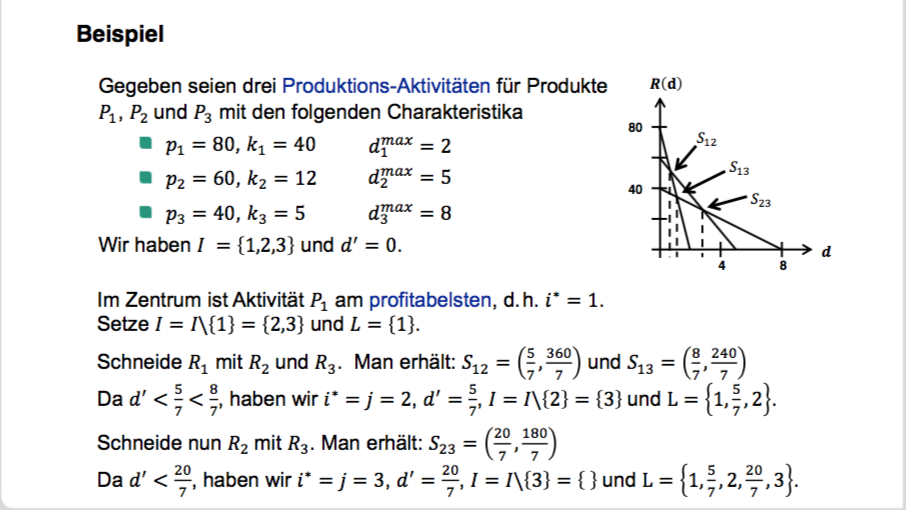
\includegraphics[width=\textwidth]{Images/Theorie_der_Boden_und_Flaechennutzung_BSP(1).png}
          % \caption{}
          % \label{}
        \end{figure}

        \begin{figure}[htbp]
          \centering
          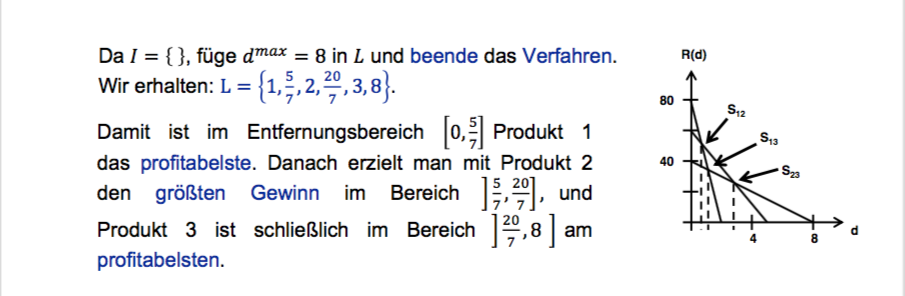
\includegraphics[width=\textwidth]{Images/Theorie_der_Boden_und_Flaechennutzung_BSP(2).png}
          % \caption{}
          % \label{}
        \end{figure}

      \begin{exmp}
        \color{blue}{Aufgabe 3}
      \end{exmp}


    % subsection theorie_der_boden_und_fla_chennutzung (end)

  % section volkswirtschaftliche_standortmodelle (end)

  \section{Deskriptive überbetriebliche Standortmodelle} % (fold)
  \label{sec:deskriptive_berbetriebliche_standortmodelle}
  
    \par Sowohl Prülisten- als auch Rangfolge-Verfahren bestimmen den besten Standort für eine neue Einrichtung basierend auf Standortfaktoren.

    \subsection{Prüflisten-Verfahren} % (fold)
    \label{sub:pr_flisten_verfahren}

      \par Vorgehensweise:

      \begin{itemize}
        \item Zusammenstellung der dem jeweiligen Problem angemessenen Standort-
faktoren. Bei dieser Aufstellung bedarf es großer Umsicht.
        \item Für jeden, der als relevant erachteten Standortfaktoren, ist zu überprüfen und entsprechend zu kennzeichnen, z. B. durch ein Kreuz, an welchem Standort der Faktor küntig am besten erfüllt sein wird.
      \end{itemize}

      \par Bei dieser Vorgehensweise werden einige Standorte mehrere Kennzeichnungen auf sich vereinen und deshalb als besonders günstig erscheinen, während andere möglicherweise leer ausgehen.

      \begin{note}\label{rem:Prüflisten-Verfahren}
        Wähle den Standort mit meisten Kreuze
      \end{note}

      \begin{exmp}
        
      \end{exmp}

      \begin{figure}[htbp]
        \centering
        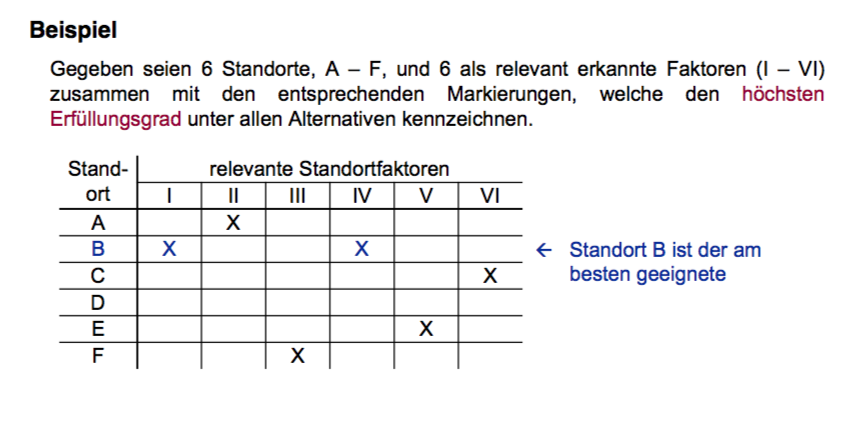
\includegraphics[width=\textwidth]{Images/Prueflisten_Verfahren_BSP.png}
        \caption{Prüflisten-Verfahren Bsp}
        % \label{}
      \end{figure}
    
    % subsection pr_flisten_verfahren (end)

    \subsection{Rangfolge-Verfahren} % (fold)
    \label{sub:rangfolge_verfahren}

      \par Vorgehensweise:

      \begin{itemize}
        \item Zusammenfassung der dem Problem angemessenen Standortfaktoren
        \item Ermittlung einer Gewichtungszahl für jeden Standortfaktoren
        \item Finde die höchste Gesamtwertigkeit
      \end{itemize}

      \begin{exmp}
        
      \end{exmp}

      \begin{figure}[H]
        \centering
        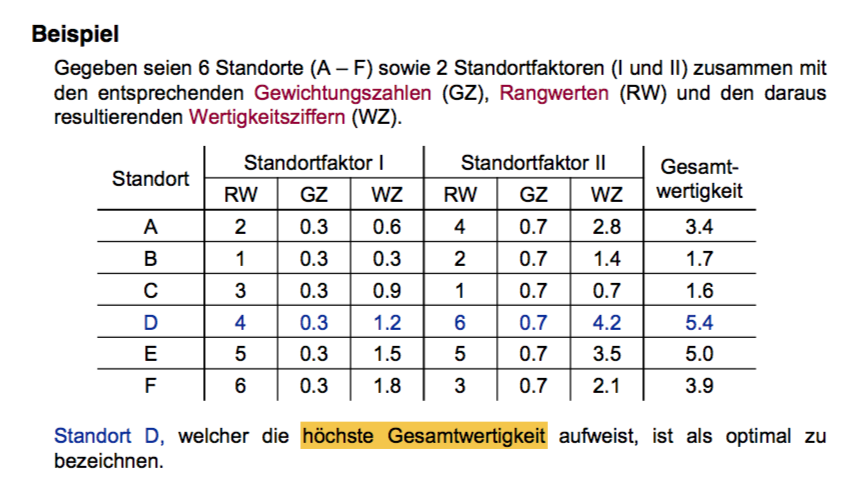
\includegraphics[width=\textwidth]{Images/Rangfolgen_Verfahren_BSP.png}
        \caption{Rangfolge-Verfahren Bsp}
        % \label{fig:label}
      \end{figure}

    
    % subsection rangfolge_verfahren (end)

  % section deskriptive_berbetriebliche_standortmodelle (end)

  \section{Standortplanung unter Wettbewerb} % (fold)
  \label{sec:standortplanung_unter_wettbewerb}

    \par Ziel: eine oder mehrere neue Einrichtung so zu platzieren, dass der Marktanteil und Gewinn der eigenen Firma maximiert wird.

    \subsection{Modelle mit vollständiger Zuordnung} % (fold)
    \label{sub:modelle_mit_vollst_ndiger_zuordnung}

      \par Der Bedarf jedes Kunden wird von genau einer Einrichtung vollständig befriedigt. (
      Bei diesen Modellen lässt sich für jeden Kunden eindeutig entscheiden, welche Einrichtung für ihn die Beste oder Attraktivste ist.)

      \begin{defn}
        \textbf{Indifferenzmenge} \\
        die Menge aller Punkte, welche gleichweit von den beiden Standorten $x_A$ und $x_B$ entfernt liegen

        \begin{equation}
          IS_{AB} := \{x \in \mathbb{R} | l_2(x;x_A) = l_2(x; x_B)\}
        \end{equation}
      \end{defn}
      \subsubsection{Voroni-diagramm} % (fold)
         \label{ssub:voroni_diagramm}

          \begin{exmp}
            \color{blue}{Aufgabe 5}
          \end{exmp}
         
         % subsubsection voroni_diagramm (end)   
    % subsection modelle_mit_vollst_ndiger_zuordnung (end)

    \subsection{Modelle mit partieller Aufteilung} % (fold)
    \label{sub:modelle_mit_partieller_aufteilung}

      \par Bei diesen Modellen verteilen die Kunden ihre Nachfrage anteilig auf mehrere Einrichtungen.

      \subsubsection{Gravitions-Modelle (Das Modell von Huff)} % (fold)
      \label{ssub:gravitions_modelle_}

      \begin{defn}
        \textbf{Anziehungskraft der Einrichtung $E$ auf den Kunden $K$}
      \end{defn}
      
      

      \begin{equation}
        A(E, K) = \frac{w_E}{d(K,E) ^ r}
      \end{equation}

      \begin{itemize}
        \item $w_E$: Größe der Einrichtung $E$ an diesem Standort
        \item $d(K, E)$: die Entfernung vom Kunden $K$ zum Standort der Einrichtung $E$
        \item $r$: eine Potenz (Verfallskonstante) für die Entfernung
      \end{itemize}

      \par \textbf{Die Wahrscheinlichkeit $P$}, dass ein Kunde eine Einrichtung an einem bestimmten Standort besucht, berechnet sich nach diesem Modell folgendermaßen:

      \begin{equation}
        P(E, K) = \frac{A(E, K)}{\sum_{\text{alle} \bar{E}}A(\bar{E}, K)}
      \end{equation}

      \begin{defn}
        \textbf{Indifferenzmege zweier Einrichtungen}\\
        die Menge alle Punkte, welche beide Einrichtungen mit derselben Wahrscheinlichkeit aufsuchen.
      \end{defn}

      \par \textbf{Der Anteil der Nachfrage eines Kunden}, welcher auf eine bestimmte Einrichtung entfällt, ergibt sich aus dem Produkt der Gesamtnachfrage des Kunden mit der „Besuchs“-Wahrscheinlichkeit

      \begin{equation}
        D(E, K) = D(K) \cdot P(K, E)
      \end{equation}
      \begin{itemize}
        \item $D(K)$: Gesammtnachfrage des Kunden
      \end{itemize}

      \par \textbf{Gesamtnachfrage einer Einrichtung} = Summe aller Anteile von Kundennachfragen

      \begin{equation}
        D(E) = \sum_{\text{alle } K}D(E, K)
      \end{equation}

      \par \textbf{gesamte Marktanteil der Einrichtung}:

      \begin{equation}
        MS(E) = \frac{D(E)}{\sum_{\text{alle } K}D(K)}
      \end{equation}

      \par Kriterium für Standort einer neuen Einrichtung $\bar{E}$:

      \[ \underset{\bar{E}}{\text{argmax}} \quad \text{MS}(\text{einige Firma}) = \frac{D(\bar{E}) + \sum_{\text{eigene, bereits exist. } E}D(E)}{\sum_{\text{alle } K}{D(K)}}\]

      \textbf{Zusammenfassung}

      \begin{figure}[H]
        \centering
        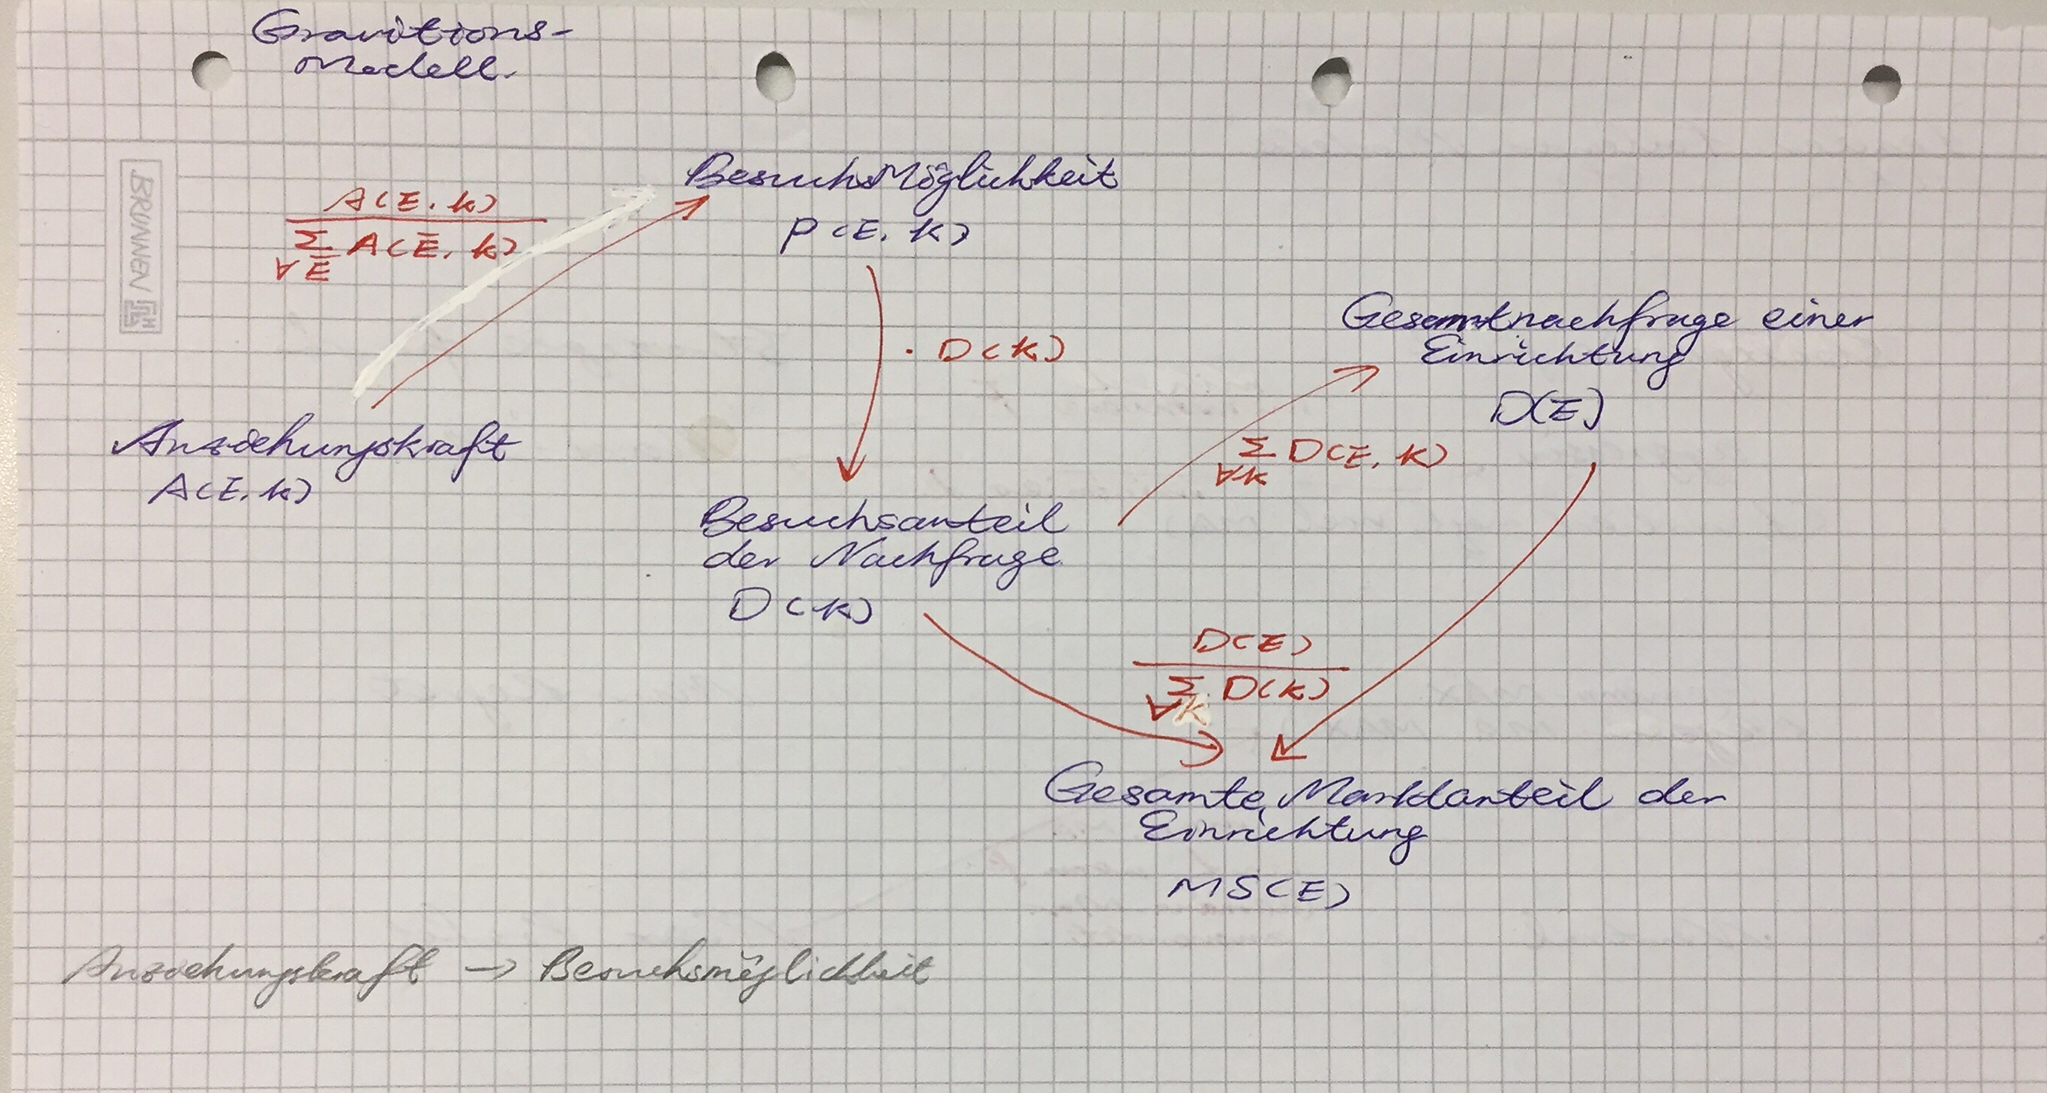
\includegraphics[width=0.95\textwidth]{Images/Gravitionsmodelle.JPG}
        \caption{Gravitionsmodelle}
        \label{fig:Gravitionsmodelle}
      \end{figure}



      \begin{exmp}
         \color{blue}{Aufgabe 4}
       \end{exmp}     
      % subsubsection gravitions_modelle_ (end)

      
    % subsection modelle_mit_partieller_aufteilung (end)

    \subsection{Leader-Follower-Modelle} % (fold)sec
    \label{sub:leader_follower_modelle}

      \subsubsection{Regeln} % (fold)
      \label{ssub:regeln}
        \begin{itemize}
          \item Bei diesen Modellen platzieren zwei Wettbewerber nacheinander neue Einrichtungen in einem (bisher unerschlossenen) Markt.
          \item Dabei wählt zuerst der Leader (Erstplatzierende) $L$ Standorte für all seine neuen Einrichtungen und danach der Follower (Zweitplatzierende) $F$.
          \item Standortwahl von $L$ und $F$ beeinflussen sich gegenseitig.
        \end{itemize}
      % subsubsection regeln (end)

      \subsubsection{Probleme / Herausforderungen} % (fold)
      \label{ssub:probleme_herausforderungen}
        \begin{itemize}
          \item \textbf{Follower $F$}\\
           Braucht sich erst auf eine Platzierungsstrategie festlegen, wenn der Erstplatzierende $L$ seine Standortwahl schon getroffen hat.
          \item \textbf{Leader $L$}\\
          Hat das Problem, dass er die Platzierungsstrategie von $F$ nicht kennt.
        \end{itemize}
      % subsubsection probleme_herausforderungen (end)

      \subsubsection{Typische Stategien für Follower $F$} % (fold)
      \label{ssub:typische_stategien_für_follower}

        \begin{itemize}
          \item \textbf{Aggressiv}\\
          Platziere neue Einrichtungen so, dass $L$ möglichst viel Marktanteil verliert. 

          \item \textbf{Gewinnmaximierend}\\
          Platziere neue Einrichtungen so, dass der eigene Marktanteil maximal wird.

          \item \textbf{Neutral}\\
          Platziere neue Einrichtungen nach anderen Kriterien.
        \end{itemize}
      
      % subsubsection typische_stategien_für_follower (end)

      \subsubsection{Verschiedene Strategien für Leader $L$} % (fold)
      \label{ssub:verschiedene_strategien_für_leader_}
      
        \begin{itemize}
          \item \textbf{Maxi-Min} \\
          $L$ platziert neue Einrichtungen so, dass sein Marktanteil maximal wird, wenn $F$ eine aggressive Strategie anwendet, d. h. $F$ das Ziel hat den Marktanteil von $L$ zu minimieren.

          \begin{framed}
            \textbf{Rechenweg}:
            \begin{enumerate}
              \item Bestimme zu jedem $L$ denjenigen Follower-Standort $\tilde{f}$, der dem Leader den geringsten Gewinn bringt, wenn der Leader bei $l$ platziert.
              \item Berechne den daraus resultierenden Marktanteil des Leaders
              \item Wähle den Standort, für den der Marktanteil des Leaders maximal wird
            \end{enumerate}
          \end{framed}
          
          \item \textbf{Min-Regret (minimales Bedauern)}\\
          $L$ platziert neue Einrichtungen so, dass, egal welche Standortentscheidung $F$ dann trifft, der Zugewinn an Marktanteil für $L$ durch eine mögliche Andersplatzierung seiner Einrichtungen (nachdem $F$ seine Wahl getroffen hat) minimal wird.

          \item \textbf{Max-Profit}\\
          $L$ platziert neue Einrichtungen so, dass ein Marktanteil maximal wird. wenn F ebenfalls eine geweinnmaximierende Strategie anwendet.

          \begin{framed}
            \textbf{Rechenweg}:
            \begin{enumerate}
              \item Bestimme zu jedem $L$ denjenigen Follower-Standort $\tilde{f}$, der dem Follower den größten Gewinn bringt, wenn der Leader bei $l$ platziert.
              \item Berechne den daraus resultierenden Marktanteil des Leaders
              \item Wähle den Standort, für den der Marktanteil des Leaders maximal wird
            \end{enumerate}
          \end{framed}

        \end{itemize}

        \textbf{Zusammenfassung}

        \begin{figure}[htbp]
          \centering
          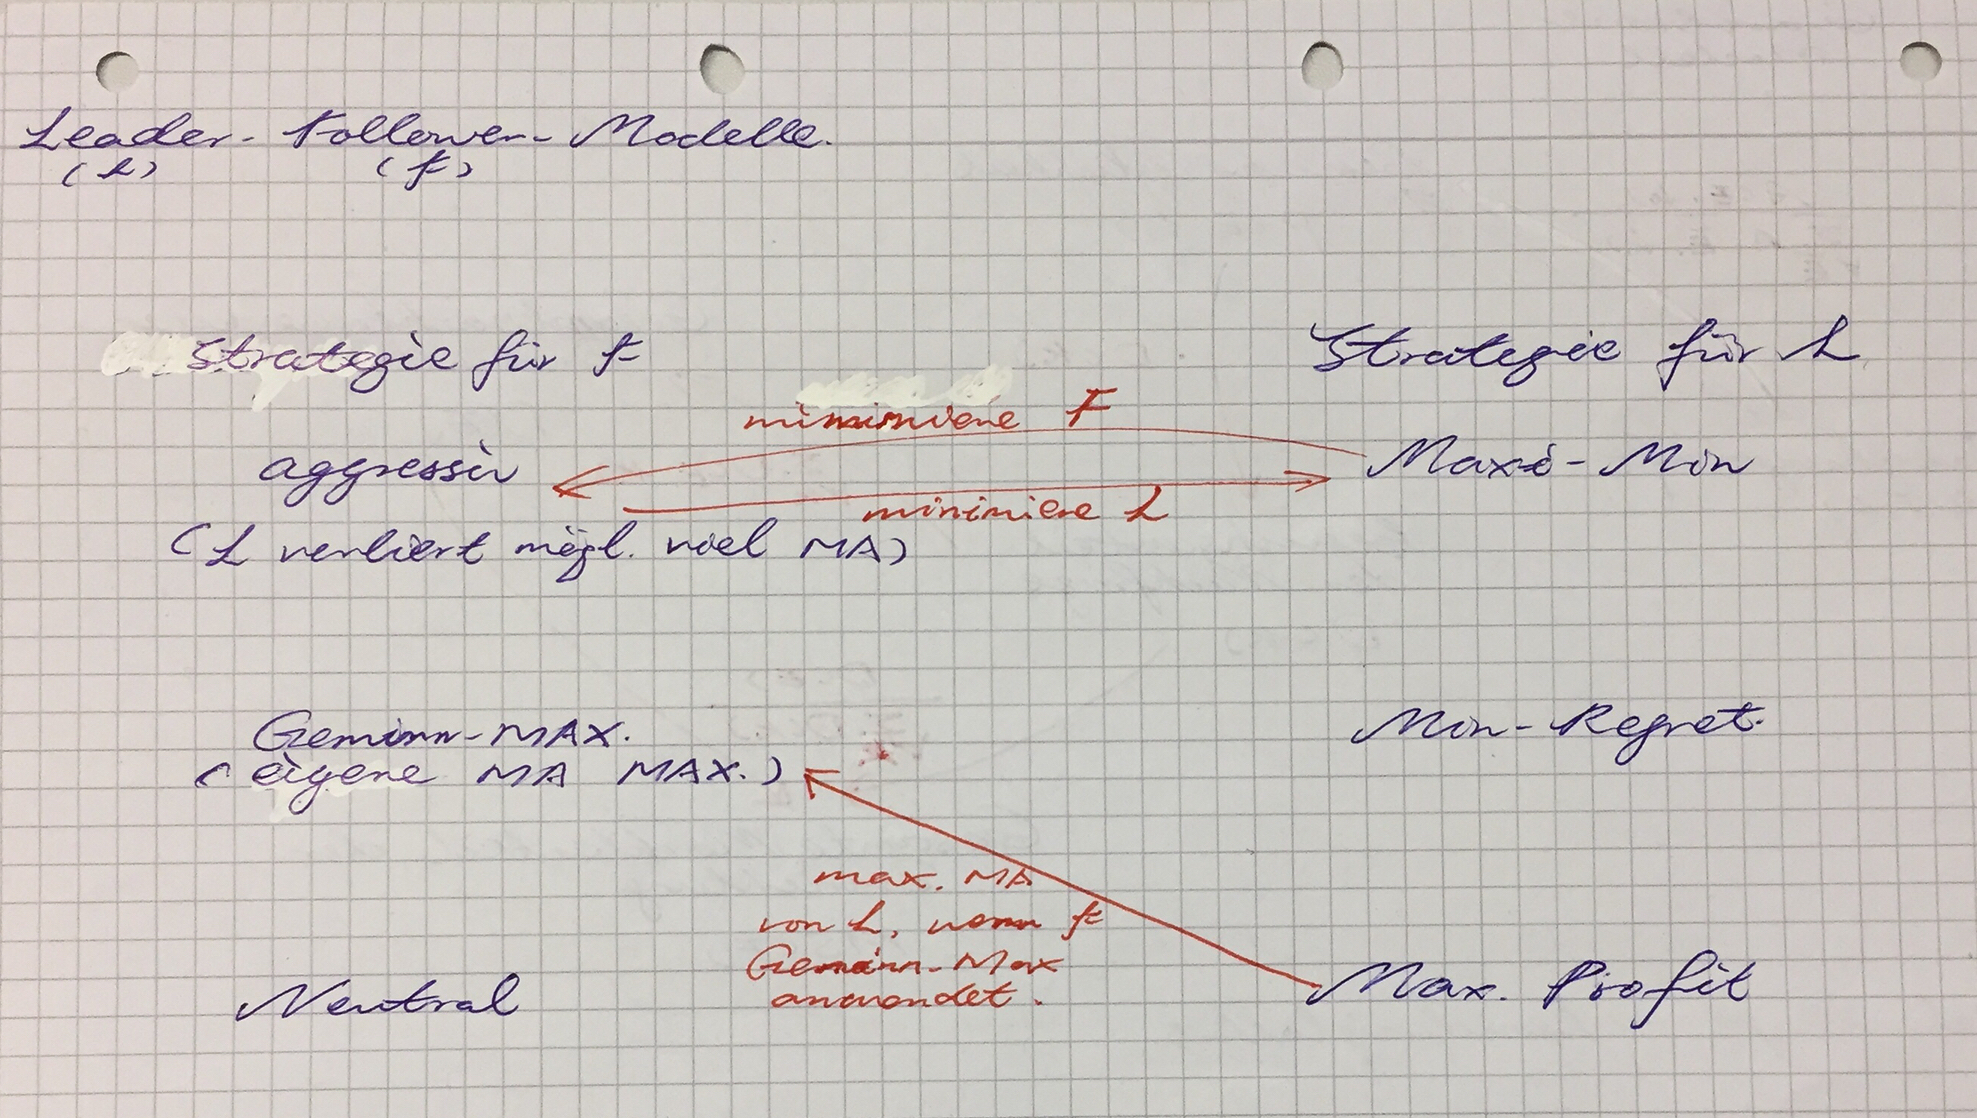
\includegraphics[width=0.95\textwidth]{Images/Leader_Follower_Modelle.JPG}
          \caption{Leader-Follower-Modelle}
          \label{fig:Leader-Follower-Modelle}
        \end{figure}

        \begin{exmp}
         \color{blue}{Aufgabe 6}
       \end{exmp} 
      % subsubsection verschiedene_strategien_für_leader_ (end)
      


    
    % subsection leader_follower_modelle (end)
  
  % section standortplanung_unter_wettbewerb (end)

% chapter volkswirtschaftliche_und_deskriptive_standortmodelle (end)



    


  \chapter{Standortplanung in der Ebene} % (fold)
\label{cha:standortplanung_in_der_ebene}

  \section{Theorie der Standortplanung} % (fold)
  \label{sec:theorie_der_standortplanung}

    \par \textbf{Grundlegende Aufgabenstellung}
    \par Platzierung ein oder mehrerer neuer Einrichtungen in Abhängigkeit bereits existierender Einrichtungen

    \par Drei Klassen von Standortproblemen:
    \begin{itemize}
      \item \textbf{Standortprobleme in der Ebene} (Einfachste, allerdings auch unrealistichste Problemklasse)
      \item \textbf{Standortprobleme auf Netzwerken} (praxisbezug viel ausgeprägter als bei planaren Standortproblemen)
      \item \textbf{Diskrete Standortprobleme} (realistischste und flexibelste Klasse von Standortproblemen)
    \end{itemize}
  
  % section theorie_der_standortplanung (end)

  \section{Begriffe und Notationen} % (fold)
  \label{sec:begriffe_und_symbole}

    \begin{defn}
      \textbf{Standorte}
      als Punkte idealisiert
    \end{defn}

    \begin{defn}
      \textbf{Neue Einrichtungen $X = {x_1, \dots, x_p}, p \geq 1$}
      \begin{itemize}
        \item dürfen überall in der Ebene platziert werden
        \item ihre Standorte werden durch Koordinaten repräsentiert
        \[ x_i = (x_{i, 1}, x_{i, 2}) \in \mathbb{R}^{2}, \forall i = 1, \dots, p\]
      \end{itemize}
    \end{defn}

    \begin{defn}
      \textbf{Existierende Einrichtungen (Kunden) $A = {a_1, \dots, a_n}$}
      \begin{itemize}
        \item werden durch eine Menge von Punkten in der Ebene repräsentiert
        \[ a_i = (a_{i, 1}, a_{i, 2}) \in \mathbb{R}^2, \forall i = 1, \dots, n\] 
        \item Jedem Kunden $a_i \in A$ wird ein positives Gewicht $w_i > 0$ zugeordnet.
      \end{itemize}
    \end{defn}
    
    \begin{defn}
      \textbf{Kosten}\\
      Lediglich Transportkosten werden berücksichtigt. Sie sind proportional zur Menge und zur zurückgelegten Entfernung.
    \end{defn}
    

    \subsection{Distanzmessung} % (fold)
    \label{sub:distanzmessung}

      \begin{defn}
        \textbf{Metrik / Distanzfunktion}
        $d: \mathbb{R}^n \times \mathbb{R}^n \rightarrow \mathbb{R}$
      \end{defn}
      \par welche für alle $ x, y, z \in \mathbb{R}^n, n \geq 1$ folgende Eigenschaften erfüllt: 
      \begin{itemize}
            \item Definitheit: $d(x,y) \geq 0 \text{ und } d(x, y) = 0 \Leftrightarrow x = y$
            \item Symmetrie: $d(x,y) = d(y, x)$
            \item Dreiecks-Ungleichung: $d(x, y) \leq d(x, z) + d(z, y)$
          \end{itemize}
    
    % subsection distanzmessung (end)

    \subsection{$l_p$-Metrik} % (fold)
    \label{sub:lp_metrik}

    \begin{equation}
      l_p(x, y) = \sqrt[p]{|x_1 - y_1| ^ p + |x_2 - y_2| ^ p}, p \geq 1
    \end{equation}
    \par \textbf{Rechtwinklige Entfernung ($l_1-$ oder Manhatten-Metrik)}

    \begin{equation}
      l_1(x, y) = |x_1 - y_1| + |x_2 - y_2|
    \end{equation}

    \par \textbf{Euklidische Entfernung ($l_2-$ oder Luftlinien-Metrik)}

    \begin{equation}
      l_2(x, y) = \sqrt{|x_1 - y_1| ^ 2 + |x_2 - y_2| ^ 2}
    \end{equation}

    \par \textbf{Quadrierte euklidische Entfernung ($l_2^2-$-Metrik)}

    \begin{equation}
      l_2(x, y) = |x_1 - y_1| ^ 2 + |x_2 - y_2| ^ 2
    \end{equation}


    \par \textbf{Tchebychev Entfernung ($l_\infty$-Metrik)}
    \begin{equation}
      l_{\infty}(x, y) = \text{max}\{\left|x_1 - y_1\right|, \left|x_2 - y_2\right|\}
    \end{equation}
    
    % subsection lp_metrik (end)

  % section begriffe_und_symbole (end)

  \section{1-Medianprobleme} % (fold)
  \label{sec:1_medianprobleme}

    \subsection{Einleitung} % (fold)
    \label{sub:einleitung}

      \subsubsection{Aufgabe} % (fold)
      \label{ssub:aufgabe}
    
      \par Platziere eine neue Einrichtung so in der Ebene, dass die Summe der gewichteten Entfernungen von dem neuen Standort zu allen Kunden minimal wird.

      \begin{equation}
        \underset{x \in \mathbb{R}^2}{\text{min}} f(x) := \sum_{i = 1}^{n}w_id(x, a_i) 
      \end{equation}

      \begin{itemize}
        \item $A = {a_1, \dots, a_n}:$ die $n$ Kunden
        \item $w_i > 0, i = 1, \dots, n$: die damit assoziierten Gewichte
        \item $x$: der gesuchte Standort der neuen Einrichtung 
        \item $d$: eine Metrik
      \end{itemize}

      \par Nenne einen Punkt $x^* \in \mathbb{R}^2$, welcher die Funktion $f(x)$ minimiert ($f(x^*) \leq f(x), \forall x \in \mathbb{R}^2$), \textbf{optimal}.

      \par Bezeichne die Menge aller optimalen Punkte der Funktion $f(\cdot)$ mit $\mathcal{X}^*(f)$.

      % subsubsection aufgabe (end)

      \subsubsection{Dominanzkriterium} % (fold)
      \label{ssub:dominanzkriterium}

        \par Gilt für einen Kunden $a_k$ mit zugehörigem Geweicht $w_k$, dass 
        \[w_k \geq \frac{1}{2}\sum_{i=1}^{n}w_i ,\]
        d. h. der Kunde vereinigt mindestens die Hälfte aller Gewichte auf sich, so ist der Standort des Kunden $a_k$ eine optimale Lösung des Problems.
      
      % subsubsection dominanzkriterium (end)

    % subsection einleitung (end)

    \subsection{1-Medianprobleme mit $l_1$-Metrik} % (fold)
    \label{sub:1_medianprobleme_mit_l1_Metrik}
    
      \par \textbf{Zielfunktion}

      \begin{equation}
        \begin{aligned}
            f(x) &= \sum_{i=1}^{n}w_il_1(x, a_i) \\
                 &= \sum_{i=1}^{n}w_il_1(\left|x_1 - a_{i,1}\right| + \left|x_2 - a_{i,2}\right|) \\
                 &= \underbrace{\sum_{i=1}^{n}w_il_1(\left|x_1 - a_{i,1}\right|)}_{=: f_1(x_1)} + \underbrace{\sum_{i=1}^{n}w_il_1(\left|x_2 - a_{i,2}\right|}_{=:f_2(x_2)}
        \end{aligned}
      \end{equation}

      $\rightarrow$ Die ursprüngliche Aufgabe reduziert sich auf das Lösen zweier 1-dimensionaler Probleme, sogenannter ``Probleme auf der Linie''.

      \subsubsection{Das 1-Medianproblem mit $l1$-Metrik auf der Linie} % (fold)
      \label{ssub:das_1_medianproblem_mit_metrik_auf_der_linie}
      
      \[\underset{x \in \mathbb{R}}{\text{min}} f(x) := \sum_{i= 1}{n}w_i\left|x - a_i\right|\]

      \begin{algorithm}[H]
        \caption{Lösungsverfahren für das 1-Medianproblem mit $l1$-Metrik auf der Linie}
        % \textbf{Input}: Anzahl Suchrichtungen $K, \beta, V, p$
        \begin{algorithmic}[1]
          % \Procedure{MyProcedure}{}
          \State Berechne die Summe $W$ aller Gewichte $W:=\sum_{i= 1}{n}w_i$
          \If (Es exist. ein $w_k \geq \frac{1}{2}W$)
            \State Der Kundenstandort $a_k$ ist eine optimale Lösung, $x^* = a_k$
            \State Stopp
          \Else
            \State Sortiere die Kundenstandorte $a_1, \dots, a_n$ nach monoton wachsenden Koordinaten $a_{i_1} \leq a_{i_2} \leq \dots \leq a_{i_n}$
            \State Bestimme unter Berücksichtigung einer zu den Kundenstandorten analogen Sortierung der Gewichte dasjenige $h$, für welches folgendes gilt:
            \[\sum_{j=1}^{h-1}w_{i_j} < \frac{1}{2}W \text{ und } \sum_{j=1}^{h}w_{i_j} \geq \frac{1}{2}W\] (die Gewichte der Reihe nach so lange aufsummiert, bis diese Summe gerade eben mehr als die Hälfte der gesamten Gewichte umfasst.)
            \State $x^* = a_{i_h}$ ist die Koordinate eines optimalen Standorts, d.h. $\mathcal{X}^*(f) = \left\{a_{i_h}\right\}$
          \EndIf
          % \EndProcedure
        \end{algorithmic}
        % \textbf{Output:} 
      \end{algorithm}

      \begin{exmp}
        
      \end{exmp}

      \begin{figure}[H]
        \centering
        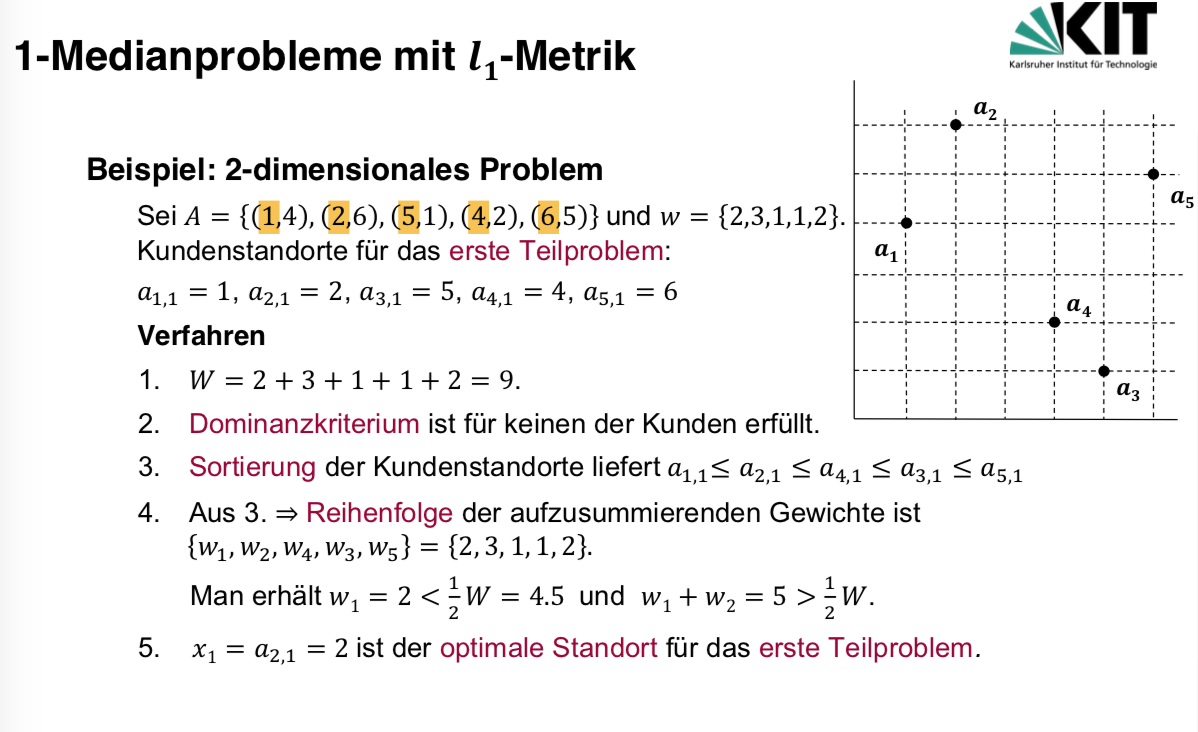
\includegraphics[width=0.95\textwidth]{Images/das_1_medianproblem_mit_metrik_auf_der_linie_Bsp(1).png}
        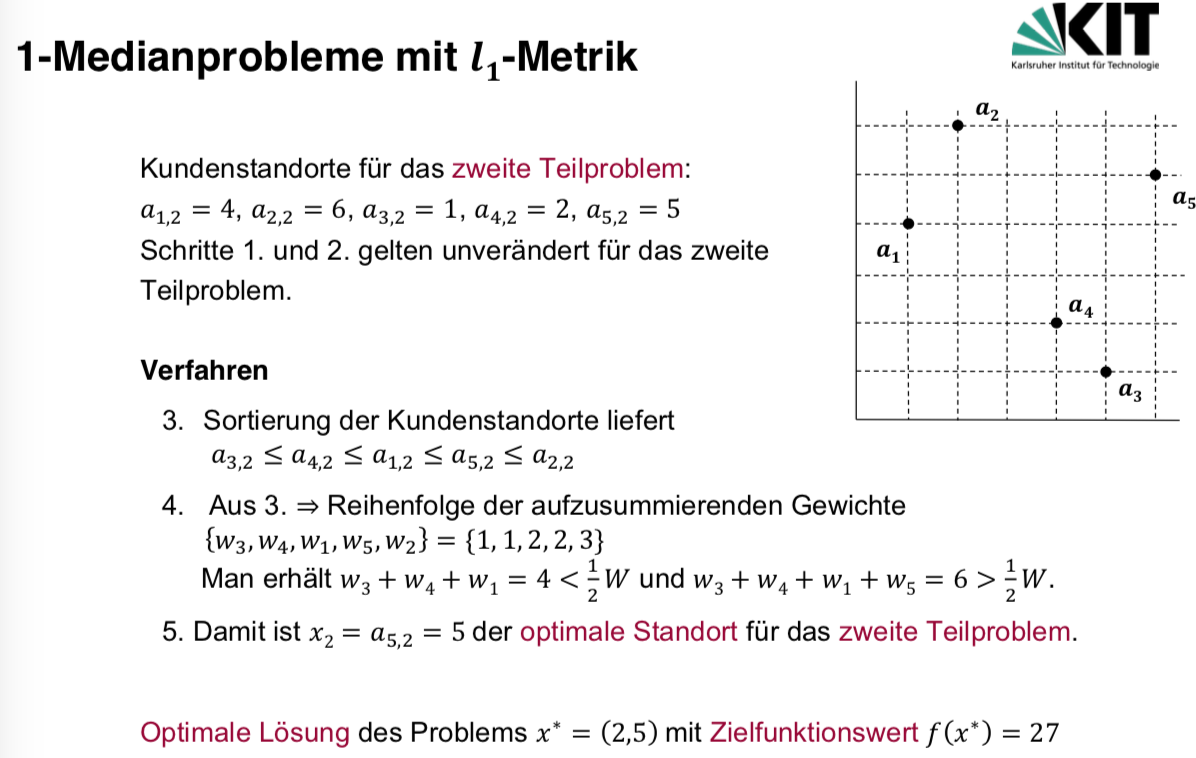
\includegraphics[width=0.95\textwidth]{Images/das_1_medianproblem_mit_metrik_auf_der_linie_Bsp(2).png}
        \caption{das $1$ medianproblem mit metrik auf der linie}
        \label{fig:das_1_medianproblem_mit_metrik_auf_der_linie}
      \end{figure}

      \textbf{Restriktive Standortprobleme mit verbotenes Gebiet R}

      \par potentielle Standorte: Schnittpunkte der achsenparallelen Geraden durch Kunden mit verboten Gebiet

      \begin{exmp}
        \color{blue}{Aufgabe 7(b)}
      \end{exmp}


      % subsubsection das_1_medianproblem_mit_metrik_auf_der_linie (end)

    % subsection 1_medianprobleme_mit_ (end)

    \subsection{1-Medianprobleme mit ${l_2}^{2}$-Metrik} % (fold)
    \label{sub:1_medianprobleme_mit_l2^2_Metrik}

    \par \textbf{Zielfunktion}

    \begin{equation}
      \begin{aligned}
        f(x) &= \sum_{i=1}^{n}w_{i}l_{2}^{2}(x, a_i) \\
             &= \sum_{i=1}^{n}w_{i}l_{2}^{2}((x_1 - a_{i, 1})^2 + (x_2 - a_{i,2})^2) \\
             &= \sum_{i=1}^{n}w_{i}l_{2}^{2}(x_1 - a_{i, 1})^2 + \sum_{i=1}^{n}w_{i}l_{2}^{2}(x_2 - a_{i, 2})^2 \\
             &=: f_1(x_1) + f_2(x_2)
      \end{aligned}
    \end{equation}

    \par $f_1(x_1)$ und $f_2(x_2)$ sind differenzierbar.

    \par Ableiten nach $x_1$ bzw. $x_2$ und Nullsetzen der jeweiligen Ableitung ergibt:

    \begin{equation*}
      \underbrace{x^*}_{Schwerpunkt} = \left(\frac{\sum_{i=1}^{n}w_ia_{i,1}}{\sum_{i=1}^{n}w_i}, \frac{\sum_{i=1}^{n}w_ia_{i,2}}{\sum_{i=1}^{n}w_i} \right)
    \end{equation*}
    
    % subsection 1_medianprobleme_mit_ (end)

    \subsection{1-Medianprobleme mit $l_2$-Metrik} % (fold)
    \label{sub:1_medianprobleme_mit_l2_Metrik}

      \par \textbf{Zielfunktion}
      \begin{equation}
        f(x) = \sum_{i=1}^{n}w_il_2(x, a_i) = \sum_{i=1}^{n}w_i\sqrt{(x_1 - a_{i,1})^2 + (x_2 - a_{i,2})^2}
      \end{equation}

      \par Die Zielfunktion ist nicht zerlegbar!

      \par \textbf{Verschärftes Dominanzkriterium}

      \par Der Standort $a_j$ eines Kunden ist optimal, falls

      \begin{equation}
        \gamma(a_j) := l_2(\sum_{i=1, i \neq j} w_i \frac{a_j - a_i}{l2(a_j, a_i)}, \mathbf{0}) \leq w_j, \mathbf{0} = (0, 0)
      \end{equation}


      \begin{algorithm}[htbp]
        \caption{Das Approximations-Verfahren von Weiszfeld}
        % \textbf{Input}: Anzahl Suchrichtungen $K, \beta, V, p$
        \begin{algorithmic}[1]
          % \Procedure{MyProcedure}{}
          \If {(Verschärftes Dominanzkriterium $\gamma(a_j) \leq w_j$ erfüllt)}
            \State $x^* = a_j$, \textbf{STOPP!}
          \Else
            \State $k:=0$
            \State $x^{(0)}:=\frac{\sum_{i=1}^{n}w_ia_i}{\sum_{i=1}^{n}w_i}$ (Schwerpunkt)
            \While {($\text{!}(\delta^(k+1):= \frac{f(x^{(k)}) - f(x^{(k+1)})}{f(x^{(k)})} \leq \delta$)}
              \State $x^{(k+1)} := \frac{\sum_{i=1}^{n}w_i\frac{a_i}{l_2(x^{(k)}, a_i)}}{\sum_{i=1}^{n}w_i\frac{1}{l_2(x^{(k)}, a_i)}}$
              \State $k:=k+1$
            \EndWhile
          \EndIf
          % \EndProcedure
        \end{algorithmic}
        % \textbf{Output:} 
      \end{algorithm}

          
    % subsection 1_medianprobleme_mit_ (end)
  
  % section 1_medianprobleme (end)

  \section{1-Centerprobleme} % (fold)
  \label{sec:1_centerprobleme}

    \subsection{Aufgabe} % (fold)
    \label{sub:aufgabe}

      Platziere eine neue Einrichtung so in der Ebene, dass die maximale gewichtete Entfernung von dem neuen Standort zu den Kunden minimal wird.
    
    % subsection aufgabe (end)

    \subsection{formel} % (fold)
    \label{sub:formel}
      \begin{equation}
        \underset{x \in \mathbb{R}^2}{\text{min}}g(x) \text{ mit } g(x) := \underset{i = 1, \dots, n}{\text{max}}w_id(x, a_i)
      \end{equation}
    % subsection formel (end)

    \subsection{1-Centerprobleme mit $l_1$-Metrik} % (fold)
    \label{sub:1_centerprobleme_mit_l_1_metrik}

      \par \textbf{Zielfunktion}

      \begin{equation}
        \begin{aligned}
          g(x) &= \underset{i = 1, \dots, n}{\text{max}}w_il_1{x, a_i} \\
               &= \underset{i = 1, \dots, n}{\text{max}}w_i(\left|x_1 - a_{i, 1} \right| + \left| x_2 - a_{i,2}\right|)
        \end{aligned}
      \end{equation}

      \begin{algorithm}[htbp]
        \caption{Lösungsverfahren für das $l_1$-Centerproblem}
        % \textbf{Input}: Anzahl Suchrichtungen $K, \beta, V, p$
        \begin{algorithmic}[1]
          % \Procedure{MyProcedure}{}
          \State Transformiere alle Kundenstandorte mit 
            \[
              T = \begin{pmatrix}
                1 & -1 \\
                1 & 1 
              \end{pmatrix}
            \]          
          \State Finde eine optimale Lösung $x_{\infty}^{*}$ des $l_{\infty}$-Problems mit den Kundenstandorten $A'$
          \State Erhalte eine optimale Lösimg $x^{*}$ des $l_1$-Problems: 
            \[
              x^* = x_{\infty}^* \cdot T^{-1}
            \]
          % \EndProcedure
        \end{algorithmic}
        % \textbf{Output:} 
      \end{algorithm}

      \subsubsection{1-Centerprobleme mit $l_{\infty}$-Metrik} % (fold)
      \label{ssub:_1_centerprobleme_mit_}

        \par \textbf{Zielfunktion}

        \begin{equation}
          \begin{aligned}
            g(x) &= \underset{i = 1, \dots, n}{\text{max}}w_il_{\infty}(x, a_i) \\
                 &= \underset{i = 1, \dots, n}{\text{max}}w_i(\left| x_1 - a_{i,1}\right|, \left| x_2 - a_{i,2}\right|)  
          \end{aligned}
        \end{equation}

        \subsubsubsection{Der ungewichtete Fall}

          \par Umformulierung des Problems:

          \begin{equation*}
            \underset{x \in \mathbb{R}^2}{\text{min}} \underset{i = 1, \dots, n}{\text{max}}l_{\infty}(x, a_i) \Leftrightarrow \underset{}{\text{min } z}, \text{u.d.N } l_{\infty}(x, a_i) \leq z, \forall i = 1, \dots, n
          \end{equation*}

          $\Rightarrow$ Minimiere $z$ unter der Nebenbedingung, dass die Entfernung von einem Punkt $x$ zu allen Kundenstandorten kleiner oder gleich $z$ ist ($l_{\infty(x, a_i)} \leq z, \forall i = 1, \dots, n$).


          \begin{algorithm}[H]
            \caption{Lösungsverfahren für ungewichtete 1-Centreprobleme mit $l_{\infty}$-Metrik}
            % \textbf{Input}: Anzahl Suchrichtungen $K, \beta, V, p$
            \begin{algorithmic}[1]
              % \Procedure{MyProcedure}{}
              \State Berechne für die Kundenstandorte das umschreibende Rechteck $R$. $R$ ist durch zwei gegenüberliegende Eckpunkte $(ul, or)$ eindeutig bestimmt.
              \If {($R$ ist ein Quadrat)}
                \State $x^*=$Mittelpunkt von $R$, \textbf{STOPP!}
              \Else
                \State Dehne das Rechteck $R$ entlang der kürzeren Seiten in beide Richtungen jeweils zu einem Quadrat $Q_1$ und $Q_2$ aus.  
                \State Die Verbindungslinie zwischen den Mittelpunkten $M_1$ und $M_2$ der beiden Quadrate $Q_1$ und $Q_2$ ist die optimale Lösungsmenge
                \begin{equation}
                  \mathcal{X}^*(g) = \overline{M_1M_2} = \{x \in \mathbb{R}^2: x = \lambda M_1 + (1 - \lambda)M_2, \forall \lambda \in [0, 1]\}
                \end{equation}
              \EndIf
              % \EndProcedure
            \end{algorithmic}
            % \textbf{Output:} 
          \end{algorithm}

          \begin{exmp}
            
          \end{exmp}

          \begin{figure}[H]
            \centering
            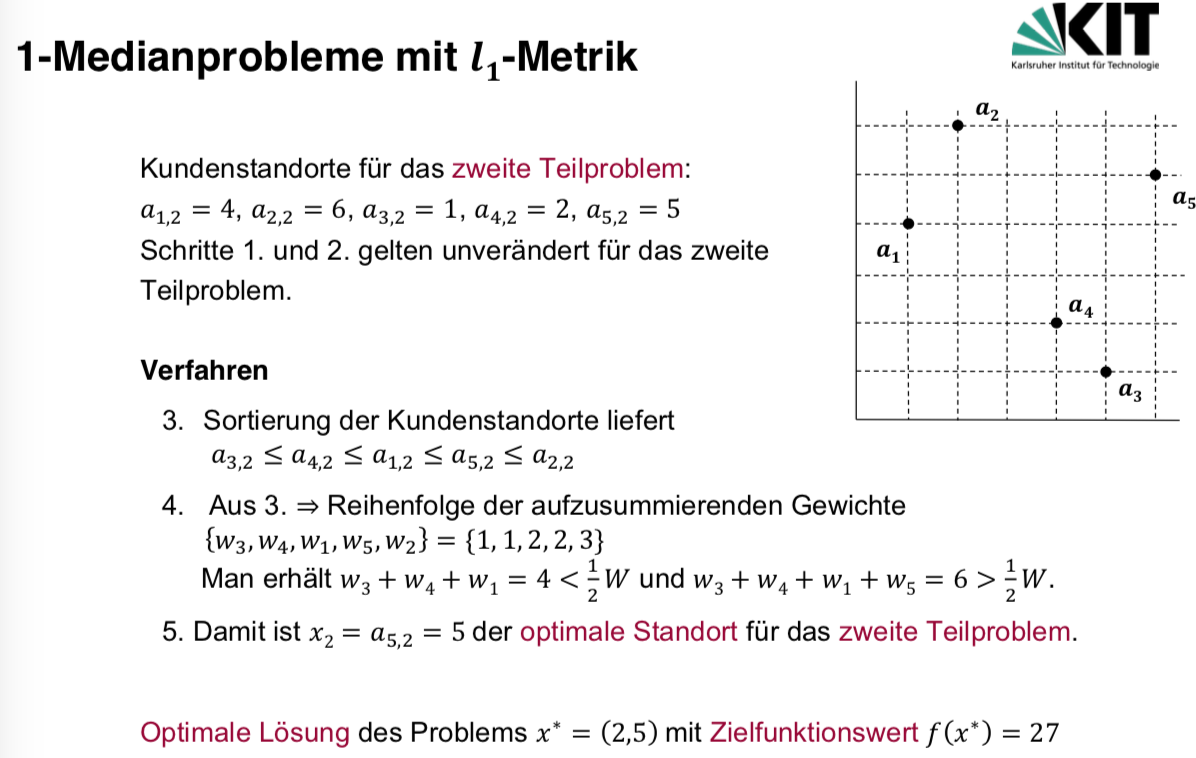
\includegraphics[width=0.95\textwidth]{Images/Loesungsverfahren_fuer_ungewichtete_1_Centreprobleme_Bsp.png}
            % \caption{Lösungsverfahren für ungewichtete 1-Centreprobleme mit $l_{\infty}$-Metrik}
            % \label{fig:Lösungsverfahren für ungewichtete 1-Centreprobleme mit l_{\infty}-Metrik}
          \end{figure}

        \subsubsubsection{Der allgemeine geweichtete Fall}

          \par \textbf{Zielfunktion}

          \begin{equation}
            \begin{aligned}
              g(x) &= \underset{i = 1, \dots, n}{\text{max}}w_i\text{max}\{|x_1 - a_{i,1}|, |x_2 - a_{i,2}|\} \\
                   &= \text{max}\{\underbrace{\underset{i = 1,\dots,n}{\text{max}}w_i|x_1 - a_{i,1}|}_{g_1(x_1}, \underbrace{\underset{i = 1,\dots,n}{\text{max}}w_i|x_2 - a_{i,2}|}_{g_2(x_2}\}
            \end{aligned}
          \end{equation}

          \par $\Rightarrow$ Das $l_{\infty}$-Centerproblem lässt sich in zwei voneinander unabhängige Teilprobleme zerlegen.


          \par \textbf{Das 1-Centerproblem mit $l_{\infty}$-Metrik auf der Linie}

          \[
            \underset{x \in \mathbb{R}}{\text{min}}g(x) \text{ mit } g(x) := \underset{i = 1, \dots, n}{\text{max}}w_i|x-a_i|
          \]
          \begin{algorithm}[H]
            \caption{Lösungsverfahren für gewichtete 1-Centreprobleme mit $l_{\infty}$-Metrik auf der Linie}
            % \textbf{Input}: Anzahl Suchrichtungen $K, \beta, V, p$
            \begin{algorithmic}[1]
              % \Procedure{MyProcedure}{}
              \State Berechne für jedes $i$ und $j$ mit $i, j \in {1, \dots, n}$
              \begin{equation*}
                \delta_{ij} = \frac{w_iw_j}{w_i+w_j}(a_j - a_i)
              \end{equation*}
              (Es gilt: $\delta_{ij} = -\delta{ji} \Rightarrow $ Es reicht aus, $\delta_{ij}$ oder $\delta_{ji}$ zu berechnen; je nachdem ob $a_i \leq a_j$ oder $a_i > a_j$)
              \State Ermittle 
              \begin{equation*}
                \delta_{pq} = max\{\delta_{ij}: i, j \in \{1, \dots, n\}\}
              \end{equation*}
              \State Optimal Lösung:
              \begin{equation*}
                z^* = \delta_{pq} \text{ und } x^{*} = \frac{w_pa_p + w_qa_q}{w_p + w_q}
              \end{equation*}
              
              % \EndProcedure
            \end{algorithmic}
            % \textbf{Output:} 
          \end{algorithm}

          \begin{exmp}
            
          \end{exmp}

          \begin{figure}[htbp]
            \centering
            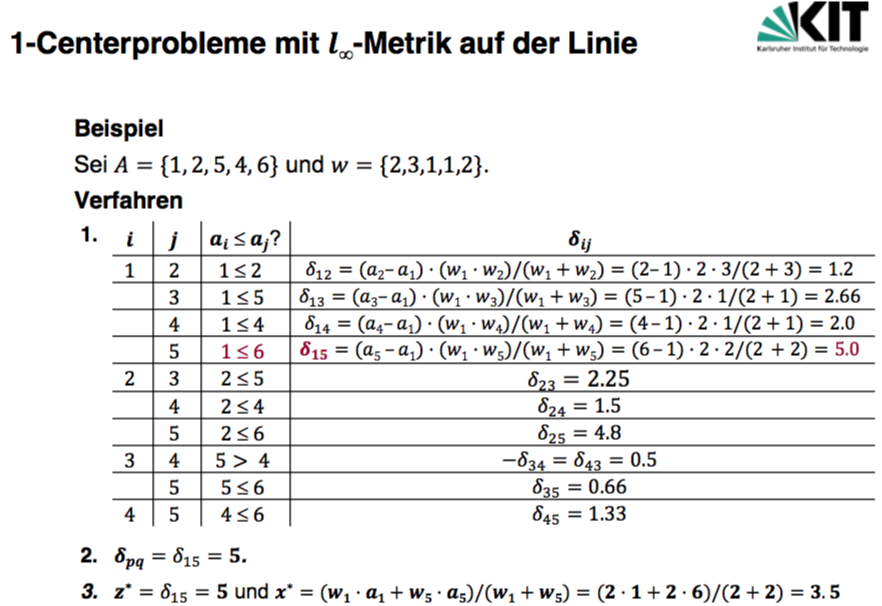
\includegraphics[width=0.95\textwidth]{Images/Das_1_Centerproblem_auf_der_Linie_Bsp.png}
            \caption{Das 1-Centerproblem mit $l_{\infty}$-Metrik auf der Linie}
            % \label{fig:Das 1-Centerproblem mit $l_{\infty}$-Metrik auf der Linie}
          \end{figure}

          \par \textbf{Kombination der Lösungen der Einzelprobleme}

          \par Seien $(x_1^*, z_1^*)$ und $(x_2^*, z_2^*)$ optimale Lösungen der zwei Teilprobleme.

          \par Dann ist $x^* := (x_1^*, x_2^*)$ eine optimale Lösungen mit $z^* = g(x^*) = \text{max}{\{g(x_1^*), g(x_2^*)\}} = \text{max}{\{z_1^*, z_2^*\}}$.

          \par Menge aller optimalen Lösungen ist

          \begin{equation*}
            \begin{aligned}
              \mathcal{X}^*(g) &= \mathcal{X}^*(g_1) \times \mathcal{X}^*(g_2) \\
                               &= [A_1^-(z^*), A_1^+(z^*)] \times [A_2^-(z^*), A_2^+(z^*)]
            \end{aligned}
          \end{equation*}
          \begin{itemize}
            \item $A^-(z) := \underset{i = 1,\dots, n}{\text{max}}a_i - \frac{z}{a_i}$
            \item $A^+(z) := \underset{i = 1,\dots, n}{\text{max}}a_i + \frac{z}{a_i}$
          \end{itemize}
      % subsubsection ungewichtete_1_centerprobleme_mit_ (end)
    
    % subsection 1_centerprobleme_mit_l_1_metrik (end)

    \subsection{1-Centerprobleme mit $l_2$-Metrik} % (fold)
    \label{sub:1_centerprobleme_mit_l_2_metrik}

      \subsubsection{Zielfunktion} % (fold)
      \label{ssub:zielfunktion}
        \begin{equation}
          \begin{aligned}
            g(x) &= \underset{i = 1,\dots, n}{\text{max}}w_il_2(x,a_i) \\
                 &= \underset{i = 1,\dots, n}{\text{max}}w_i\sqrt{(x_1 - a_{i, 1})^2 + (x_2 - a_{i,2})^2}
          \end{aligned}
        \end{equation}
      % subsubsection zielfunktion (end)

      \subsubsection{Der ungewichtete Fall: Das Kreis-Überdeckungsproblem} % (fold)
      \label{ssub:der_ungewichtete_fall_das_kreis_überdeckungsproblem}
        \par Umformulierung des Problems:

        \[
          \underset{x \in \mathbb{R}^2}{\text{min}} \underset{i = 1,\dots, n}{\text{max}}w_il_2(x,a_i) \Leftrightarrow \text{min } z, \text{u.d.N. } l_2(x, a_i) \leq z, \forall i = 1, \dots, n
        \]

        \par $\Rightarrow$ \textbf{Das minimale Kreis-Überdeckungsproblem}: Minimiere $z$ unter der Nebenbedingung, dass die Entfernung von einem Punkt $x$ zu allen Kundenstandorten kleiner oder gleich $z$ ist.

        \begin{algorithm}[H]
          \begin{algorithmic}[1]
            \caption{Enumertations-Verfahren}
              \State Berechne alle minimalüberdeckenden Kreise von zwei oder drei Kundenstandorten $a_i, a_j$ und $a_k \in A$
              \State Verwirf alle so gewonnen minimalüberdeckenden Kreise, die nicht alle Kundenstandorten überdecken.
              \State Der verbleibende MÜK (Minimal Überdeckender Kreis) ist der MÜK für alle Kundenstandorten
              % \EndProcedure
            \end{algorithmic}
          % \textbf{Output:} 
        \end{algorithm}

        \par Komplexität:$O(n^4) \rightarrow$ zu langsam!

        \begin{algorithm}[H]
          \begin{algorithmic}[1]
            \caption{Verfahren von Elzinga \& Hearn}
            \State Starte mit dem MÜK zweier beliebiger Kundenstandorten $a$ und $b$
            \State Werden alle Kunden von dem Kreis überdeckt $\Rightarrow$ Schritt 9
            \State Wähle einen Kunden $c$, der noch nicht überdeckt wird, und konstruiere den MÜK für diese drei Kunden.
            \State Werden alle Kunden von dem Kreis überdeckt $\Rightarrow$ Schritt 9.
            \State Wird der MÜK von zwei Kunden $a$ und $b$ bestimmt
              $\Rightarrow$ fahre mit $a$ und $b$ fort mit Schritt 3, 
              $\Rightarrow$ andernfalls fahre mit allen dreien fort mit Schritt 6.
            \State Wähle einen weiteren Kunden $d$, der noch nicht überdeckt wird, und konstruiere (mit Hilfe des Enumerations-Verfahrens) den MÜK für diese vier Kunden.  
            \State Werden alle Kunden von dem Kreis überdeckt $\Rightarrow$ Schritt 9
            \State Wird der MÜK von zwei Kunden $a$ und $b$ bestimmt
              $\Rightarrow$ fahre mit $a$ und $b$ fort mit Schritt 3, 
              $\Rightarrow$ andernfalls fahre mit den drei MÜK-definierenden Kunden fort mit Schritt 6.
            \State Der momentane MÜK überdeckt alle Kundenstandorte und ist somit der optimale.
              % \EndProcedure
            \end{algorithmic}
          % \textbf{Output:} 
        \end{algorithm}

        \begin{exmp}
          
        \end{exmp}

        \begin{figure}[H]
          \centering
          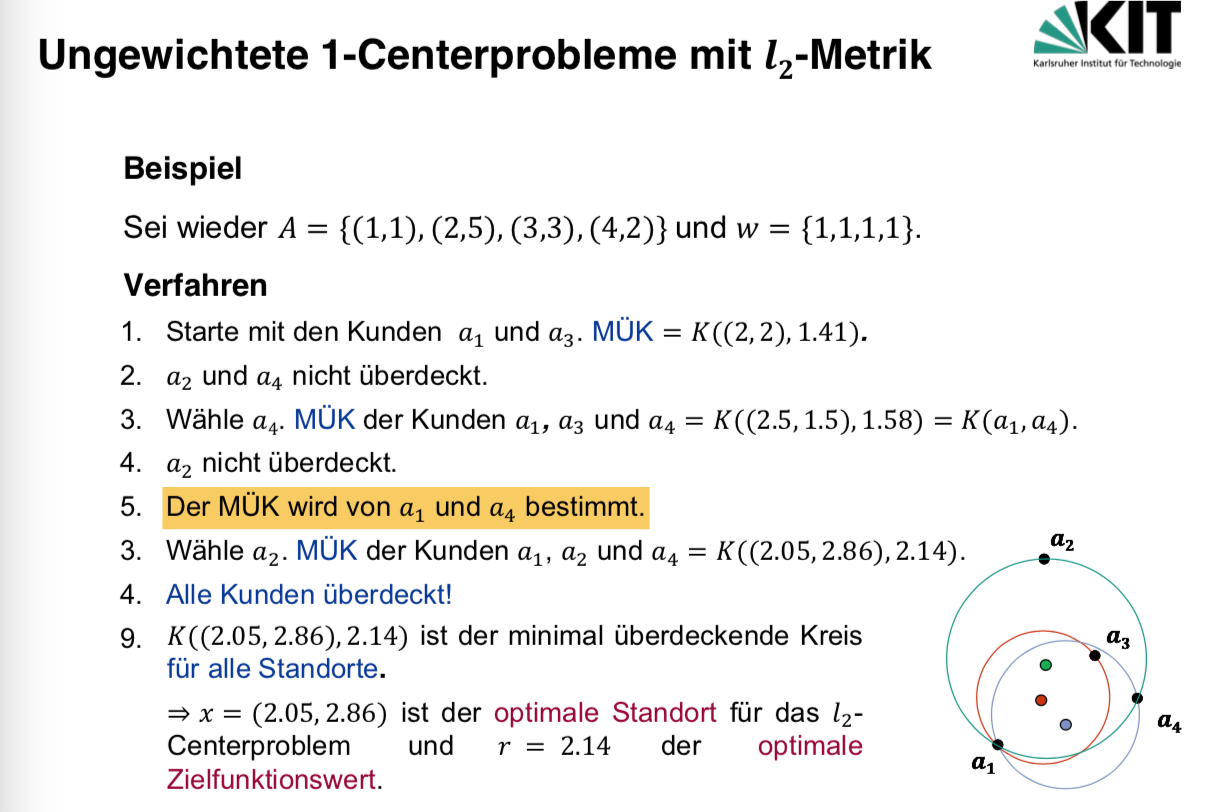
\includegraphics[width=0.95\textwidth]{Images/Verfahren_von_Elzinga_und_Hearn_Bsp.png}
          \caption{Verfahren von Elzinga \& Hearn}
          \label{fig:Verfahren von Elzinga & Hearn}
        \end{figure}

      % subsubsection der_ungewichtete_fall_das_kreis_überdeckungsproblem (end)
    
    % subsection 1_centerprobleme_mit_l_2_metrik (end)

  
  % section 1_centerprobleme (end)

  \section{Mehrstandortprobleme} % (fold)
  \label{sec:mehrstandortprobleme}

    \par Platziere $p$ neue Einrichtungen $X={x_1, \dots, x_p}, p \geq 2$ in der Ebene

    \begin{itemize}
      \item Modellen mit Interaktion
        \begin{itemize}
          \item Neue Einrichtungen bieten jeweils unterschiedlichen Service (verschiedene Güter) an.
          \item Kunden haben Nachfrage nach unterschiedlichen Serviceleistungen (Gütern) von mehreren der neuen Einrichtungen.
          \item Interaktion, z. B. Austausch von Gütern, zwischen neuen Einrichtungen erlaubt.
        \end{itemize}
      \item Zuordnungs-Modellen (Standort-Einzugsbereichs-Modellen
        \begin{itemize}
          \item Neue Einrichtungen bieten alle gleichen Service (identische Güter) an.
          \item Kunden befriedigen ihre Nachfrage von einem der neuen Standorte.
        \end{itemize}
    \end{itemize}
  
    \subsection{Modelle mit Interaktion} % (fold)
    \label{sub:modelle_mit_interaktion}

      \subsubsection{Annahmen} % (fold)
      \label{ssub:annahmen}

        \par \textbf{Nachfrage} des Kunden $i$ nach einem Service der neuen Einrichtung $k$: $w_ik$
        \par \textbf{Interaktion} zwischen zwei neuen Einrichtungen $k$ udn $l$: $s_{kl}$     
        % subsubsection annahmen (end)

      \subsubsection{Zielfunktion} % (fold)
      \label{ssub:zielfunktion}
      
        \begin{equation}
          \begin{aligned}
            \underset{X \subseteq \mathbb{R}^2, |X| = p}{\text{min}}f(X):= \sum_{i = 1}^{n}\sum_{k = 1}^{p}w{ik}d(x_k, a_i) + \sum_{k = 1}^{p - 1}\sum_{l = k + 1}^{p}s_{kl}d(x_k, x_l)    
          \end{aligned}
        \end{equation}
      % subsubsection zielfunktion (end)

      \subsubsection{Notationen} % (fold)
      \label{ssub:notationen}

        \par $x_1, \dots, x_p$ sind nun Punkte mit Koordinaten $x_{k,1}$ und $x_{k,2}, k = 1, \dots, p$

        \par $X_1:= {x_{1,1}, \dots, x_{p,1}}$ und $X_2 := {x_{1,2}, \dots, x_{p,2}}$
      
      % subsubsection notationen (end)

      \subsubsection{Das Interaktions-Modell mit $l_1$-Metrik} % (fold)
      \label{ssub:das_interaktions_modell_mit_l1_metrik}

        \par \textbf{Zielfunktion}

        \begin{equation}
          \begin{aligned}
            f(X) &= \sum_{i=1}^{n}\sum_{k=1}^{p}w_{ik}(|x_{k,1}-a_{i,1}| + |x_{k,2}- a_{i,2}|) + \sum_{k=1}^{p-1}\sum_{l=k+1}^{p}s_{kl}(|x_{k,1}-x_{l,1}|+|x_{k,2}- x_{l,2}|) \\
                 &=  \underbrace{\sum_{i=1}^{n}\sum_{k=1}^{p}w_{ik}|x_{k,1}-a_{i,1}| + \sum_{k=1}^{p-1}\sum_{l=k+1}^{p}s_{kl}|x_{k,1}-x_{l,1}|}_{=: f_1(X_1)} + \underbrace{\sum_{i=1}^{n}\sum_{k=1}^{p}w_{ik}|x_{k,2}-a_{i,2}| + \sum_{k=1}^{p-1}\sum_{l=k+1}^{p}s_{kl}|x_{k,2}-x_{l,2}|}_{f_2(X_2)}
          \end{aligned} 
        \end{equation}

        $\rightarrow$Zielfunktion zerfällt in zwei voneinander unabhängige Funktionen.

        \par \textbf{Das Interaktions-Modell mit $l_1$-Metrik auf der Linie}

        \par \textbf{Zielfunktion}

        \begin{equation}
          \sum_{i=1}^{n}\sum_{k=1}^{p}w_{ik}|x_{k}-a_{i}| + \sum_{k=1}^{p-1}\sum_{l=k+1}^{p}s_{kl}|x_{k}-x_{l}|
        \end{equation}

        \par \textbf{Umformulierung als lineares Programm}

        \begin{framed}
          \par Seien $a, b \in \mathbb{R}$ und $c, d \in \mathbb{R}_+$\\
          \par Gilt: 
          \[c \cdot d = 0 \text{ und } a - b = c - d\]
          \par Dann:
          \[|a - b| = c + d\]
          \par Ersetze:
          \[|x_k - a_i| = \alpha_{ik} + \beta_{ik} \in \mathbb{R}_+, \text{für } \alpha_{ik}, \beta_{ik} \in \mathbb{R}_+\]
          \par und 
          \[|x_k - x_l| = \gamma_{kl} + \delta_{kl} \in \mathbb{R}_+, \text{für } \in \gamma_{kl}, \delta_{kl} \in \mathbb{R}_+\]
        \end{framed}

        \par Dann:

        \begin{equation}
          \begin{aligned}
            & \underset{}{\text{min}}
            && \sum_{i=1}^{n}\sum_{k=1}^{p}w_{ik}(\alpha_{ik} + \beta_{ik}) + \sum_{k=1}^{p-1}\sum_{l=k+1}^{p}s_{kl}(\gamma_{kl} + \delta_{kl})\\
            % & & e - (s + re) \\
            & \text{u.d.N}
            & & x_k - \alpha_{ik} + \beta_{ik} = a_i, \quad \forall i = 1, \dots, n, k = 1, \dots, p\\ 
            & & & \alpha_{ik} \cdot \beta_{ik} = 0, \quad \forall i = 1, \dots, n, k = 1, \dots, p\\ 
            & & & x_k - x_l - \gamma_{kl}+ \delta_{kl} = 0, \quad \forall k, l = 1, \dots, p, k < l \\
            & & & \gamma_{kl} \cdot \delta_{kl} = 0, \quad \forall k, l = 1, \dots, p, k < l \\
            & & & \alpha_{ik}, \beta_{ik}, \gamma_{kl}, \delta_{kl} \geq 0, \quad \forall i, k, l \text{ und } x_k, x_l \in \mathbb{R}, \forall k,l
          \end{aligned}
        \end{equation}

        \begin{exmp}
          
        \end{exmp}

        \begin{figure}[H]
          \centering
          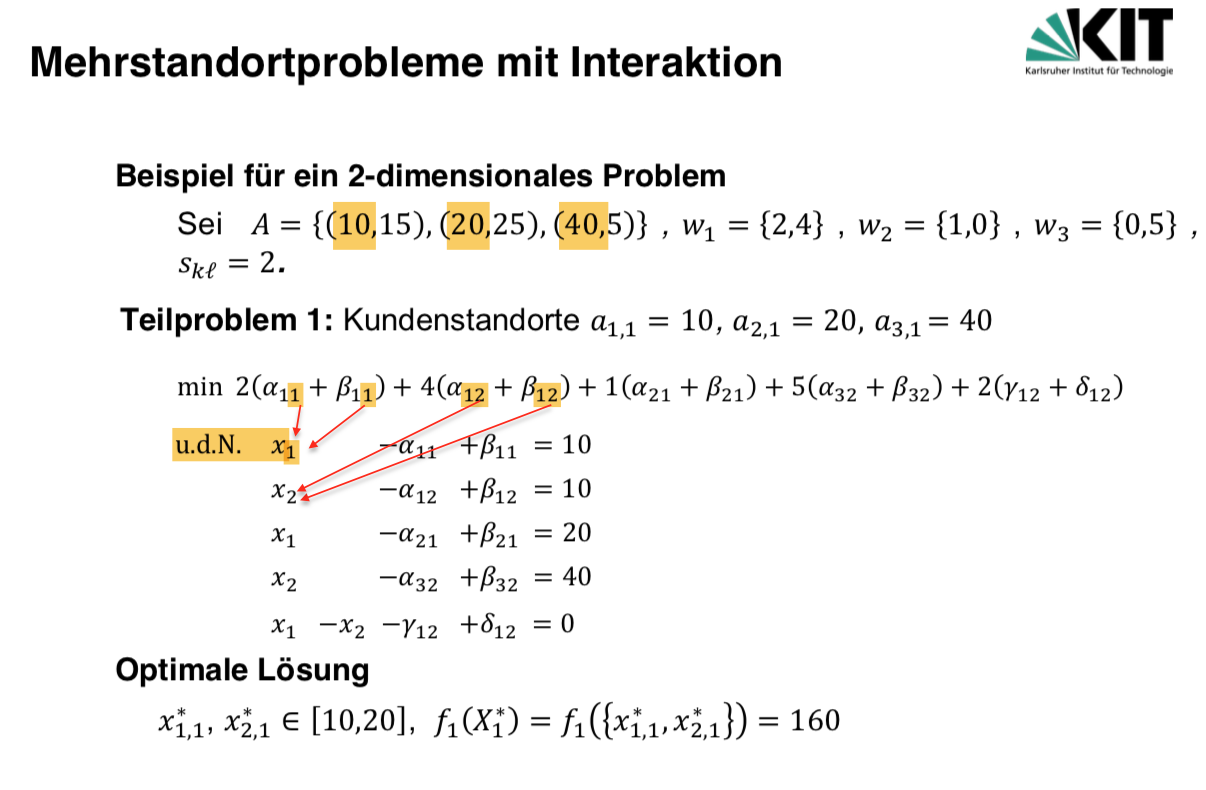
\includegraphics[width=0.95\textwidth]{Images/Mehrstandorten_Problem_mit_Interaktion_Umformulierung_Bsp.png}
          \caption{Mehrstandorten Problem mit Interaktion Umformulierung Bsp}
          \label{fig:Mehrstandorten_Problem_mit_Interaktion_Umformulierung_Bsp}
        \end{figure}
      
      % subsubsection das_interaktions_modell_mit_l1_metrik (end)
      
      \subsubsection{Das Interaktions-Modell mit $l_2$-Metrik} % (fold)
      \label{ssub:das_interaktions_modell_mit_metrik}
      
      % subsubsection das_interaktions_modell_mit_metrik (end)
    % subsection modelle_mit_interaktion (end)

    \section{Zuordnungs-Modelle} % (fold)
    \label{sub:zuordnungs_modelle}

      \begin{itemize}
        \item Neue Einrichtungen bieten alle gleichen Service (identische Güter) an.
        \item Kunden befriedigen ihre Nachfrage von einem der neuen Standorte.
      \end{itemize}

      \par \textbf{Präferenzfunktion}    
      \par Definiere eine Präferenzfunktion, welche jeden Kunden einer neuen Einrichtung zuordnet:
      \[\text{Präf}: A \rightarrow X \qquad \qquad \text{Präf}(a_i) = x_k \in X \text{ mit } d(x_k, a_i) = \underset{l=1, \dots, p}{\text{min}}d(x_l. a_i)\]

      \par ($a_i$ liegt näher bei $x_k$ als bei allen anderen Lösungspunkten; die Nachfrage von$a_i$ wird von der neuen Einrichtung $x_k$ befriedigt.)

      \par Menge aller Kunden, welche einem Standort $x_l$ zugeordnet sind
      \[A_k := \{a_i \in A | \text{Präf}(a_i) = x_k\} = \{a_i \in A | d(x_k, a_i) = d(X, a_i)\}\]

        \subsection{Das p-Median Zuordnungsproblem} % (fold)
        \label{sub:das_p_median_zuordnungsproblem}

          \par \textbf{Zielfunktion}

          \begin{equation}
            f(X) = f(\{x_1, \dots, x_p\}) = \sum_{i=1,\dots,n}w_id(X, a_i)
          \end{equation}
          \subsubsection{Das p-Median Zuordnungsproblem mit $l_1$-Metrik} % (fold)
          \label{ssub:das_p_median_zuordnungsproblem_mit_l1_metrik}
            
            \par \textbf{Zielfunktion}

            \[f(X) = \sum_{i = 1, \dots, n}w_i \underset{k = 1, \dots, p}{\text{min}\{|x_{k,1} - a_{i,1}| + {x_{k,2} - a_{i,2}}\}}\]

            \par Definiere

            \[
              y_k := 
              \begin{cases}
                1 & \text{falls der Schnittpunkte } s_k \text{ Teil der optimalen Lösung ist}, k = 1, \dots, |S|\\
                0 & sonst 
              \end{cases}\\ 
            \]
            \[
               x_{ik} := 
              \begin{cases}
                1 & \text{falls Kunde } i \text{ dem Schnittpunkte } s_k \text{ zugeordnet ist.}, i = 1, \dots n, k = 1, \dots, |S| \\
                0 & sonst
               \end{cases} 
            \]
            \[
              c_{ik} := w_il_1(a_i, s_k), i = 1, \dots n, k = 1, \dots, |S|
            \]

               
            

            \par \textbf{Modell}

            \begin{equation}
              \begin{aligned}
                & \underset{}{\text{min}}
                && \sum_{i=1,\dots, n}\sum_{k=1, \dots, |S|}c_{ik}x_{ik}\\
                % & & e - (s + re) \\
                & \text{u.d.N}
                & & \sum_{k = 1, \dots, p}x_{ik} = 1, \forall i \quad \text{Jeder Kunde i wird einem Schnittpunkte zugeordnet}\\
                & & & \sum_{k = 1, \dots, |S|}y_k = p \quad \text{(p Schnittpunkte werden ausgewählt)}\\ 
                & & & x_{ik} \leq y_k , \forall i, \forall k \quad \text{(Kunde i darf nur eineme ausgewählten Schnittpunkt k zugeordnet werden)}\\
                & & & x_{ik}, y_{k} \in \{0, 1\}
              \end{aligned}
              \label{p-Median Zuordnungsproblem}
            \end{equation}

            \par Ganzzahliges lineares Programm \\
            $\rightarrow$ Lässt sich mit Branch \& Bround-Verfahren lösen.




          % subsubsection das_p_median_zuordnungsproblem_mit_l1_metrik (end)

          \subsubsection{Das Zuordnungsproblem mit $l_2$-Metrik} % (fold)
          \label{ssub:das_zuordnungsproblem_mit_metrik}
          
            \par \textbf{Zielfunktion}         

            \begin{equation}
               f(X) = \sum_{i = 1, \dots, n}w_i\underset{k=1,\dots,p}{\text{min}}l_2(x_k, a_i)
            \end{equation} 

            \begin{algorithm}[H]
          \begin{algorithmic}[1]
            \caption{Das Verfahren von Cooper}
            \State Wähle eine Startlösung $X^{0} = {x_1^{(0)}, \dots, x_p^{(0)}}$ setze $l := 0$
            \While{(!($\delta^{(l+1)}:=\frac{f(X^l)-f(X^{l+1})}{f(X^{(l)})} \leq \delta$ für ein $\delta > 0$))}
              \State \textbf{Zuordnungsschritt (allocation)}: Berechne für $X^{(l)}$ die Partition $Pa^{(l)} = \{A_1^{(l)}, \dots, A_p^{(l)}\}$ der Kundenstandorte
              \State \textbf{Platzierungsschritt (location)}: Bestimme die optimale Lösung $X_k^{(l+1)}$ des 1-Standortproblems mit Kunden $A_k^{(l)}$. Setze $X^{(l+1)}:= \{x_1^{(l+1), \dots, x_p^{(l+1)}}\}$
              \State $l:=l+1$
            \EndWhile
              % \EndProcedure
            \end{algorithmic}
          % \textbf{Output:} 
        \end{algorithm}


          % subsubsection das_zuordnungsproblem_mit_metrik (end)


        
        % subsection das_p_median_zuordnungsproblem (end)
    % section zuordnungs_modelle (end)

  % section mehrstandortprobleme (end)


% chapter standortplanung_in_der_ebene (end)




  \section{Standortplanung auf Netzwerken} % (fold)
    \label{sec:standortplanung_auf_netzwerken}

      \subsection{Graphentheorie} % (fold)
      \label{sub:graphentheorie}
      
      % subsection graphentheorie (end)

      \subsection{1-Medianprobleme} % (fold)
      \label{sub:1_medianprobleme}

        \subsubsection{1-Medianprobleme auf allgemeinen Graphen} % (fold)
        \label{ssub:1_medianprobleme_auf_allgemeinen_graphen}
        
        % subsubsection 1_medianprobleme_auf_allgemeinen_graphen (end)

        \subsubsection{1-Medianprobleme auf Bäume} % (fold)
        \label{ssub:1_medianprobleme_auf_b_ume}
        
        % subsubsection 1_medianprobleme_auf_b_ume (end)
      
      % subsection 1_medianprobleme (end)

      \subsection{1-Centerprobleme} % (fold)
      \label{sub:1_centerprobleme}
      
        \subsubsection{1-Centerprobleme auf allgemeinen Graphen} % (fold)
        \label{ssub:1_centerprobleme_auf_allgemeinen_graphen}
        
        % subsubsection 1_centerprobleme_auf_allgemeinen_graphen (end)

        \subsubsection{1-Centerprobleme auf Bäume} % (fold)
        \label{ssub:1_centerprobleme_auf_b_ume}
        
        % subsubsection 1_centerprobleme_auf_b_ume (end)

      % subsection 1_centerprobleme (end)

      \subsection{Mehrstandortprobleme} % (fold)
      \label{sub:mehrstandortprobleme}
      
      % subsection mehrstandortprobleme (end)
    
    % section standortplanung_auf_netzwerken (end)

  
\chapter{Diskrete Standortplanung} % (fold)
\label{cha:diskrete_standortplanung}

  \section{Klassifikation diskreter Standortprobleme} % (fold)
  \label{sec:klassifikation_diskreter_standortprobleme}

    \par \textbf{Planungshorizont}
    \par Anzahl der Zeitperioden (z. B. Monate, Jahre) im Planungszeitraum.
    \begin{itemize}
      \item Statische (Ein-Perioden) Modelle\\
      Standortentscheidungen werden zu Beginn des Planungshorizontes getroffen
      \item Dynamische (Mehr-Perioden) Modelle\\
      Entscheide wo und wann, d. h. in welcher Periode, Einrichtungen platziert werden.
    \end{itemize}

    \par \textbf{Einrichtungstypen}
    \par Unterscheide verschiedene Ausprägungen von Einrichtungen,

    \par \textbf{Produktaggregation}
    \par Ist nur ein Produkt oder sind mehrere Produkte mit unterschiedlichen Charakteristiken zu planen?

    \par \textbf{Stufigkeit}
    \par Anzahl der Stufen des Distributionsnetzwerks.
    \begin{itemize}
      \item Einstufige Modelle\\
      Güterverteilung über eine Transportstufe (z. B. Lager$\rightarrow$Händler). Standortentscheidung nur auf einer Ebene (z. B. Lager).
      \item Mehrstufige (hierarchische) Modelle\\
      Güterverteilung über mehrere Transportstufen (z. B. Werk$\rightarrow$Lager$\rightarrow$Händler).
    \end{itemize}

    \par \textbf{Interaktion}
    \par Interaktion zwischen Einrichtungen desselben Typs möglich, z. B. Transporte zwischen Warenhäusern.

    \par \textbf{Unsicherheit}
    \begin{itemize}
      \item Deterministische Modelle\\
      alle Daten und Parameter sind vollständig bekannt
      \item Probabilistische (stochastische) Modelle\\
      manche Daten und Parameter sind unsicher
    \end{itemize}

    \par \textbf{Flussrichtung}
    \begin{itemize}
      \item Distributionslogistik\\
      Waren fließen von Werken/Lieferanten zu den Lagern/Kunden
      \item Entsorgungslogistik (Reverse Logistics)\\
      Waren fließen von Kunden zu Recyclinganlagen, Deponien
    \end{itemize}

    \par \textbf{Kapazitätsrestriktionen}
    \par Beschränken die Mengen, welche produziert, transportiert, umgeschlagen etc. werden können.

    \par \textbf{Transportmodus}
    \begin{itemize}
      \item Touren-Belieferungen\\ 
      Auslieferungen von einer übergeordneten Einrichtung zu untergeordneten Einrichtungen (oder umgekehrt) werden zu Touren gebündelt.
      \item Direkt-Belieferungen\\ 
      Auslieferungen von übergeordneten zu untergeordneten Ebenen geschehen direkt und ohne Umwege.
    \end{itemize}
    
    \par \textbf{}


  
  % section klassifikation_diskreter_standortprobleme (end)

  \section{Das Warehouse Location Problem (WLP)} % (fold)
  \label{sec:das_warehouse_location_problem_}

    \par Auch als \textbf{Uncapacitated Facility Location Problem (UFLP)} oder \textbf{Simple Plant Location Problem (SPLP)} bekannt.

    \par \textbf{Modell-Annahmen}
    \begin{itemize}
      \item statisch, einstufig, unkapazitiert, deterministisch
      \item ein Produkt, Direkt-Belieferung, ein Einrichtungstyp, keine Interaktion
    \end{itemize}

    \par \textbf{Gegeben}
    \begin{itemize}
      \item Menge von Kunden $I = \{1, \dots, n\}$ mit Bedarfen $b_i, i = 1, \dots, n$
      \item Menge potentieller Standorte $J = \{1, \dots, m\}$ für neue Einrichtungen
      \item Kosten $t_{ij}$ für den Transport einer Mengeneinheit vom potentiellen Standort $j \in J$ zu einem Kunden $i \in I$.
      $\rightarrow$ Gesamtkosten zur Belieferung des Kunden $i$ vom Standort $j$: $c_{ij} = b_i \cdot t_{ij}$ \\$\rightarrow$ Kostenmatrix $C = (c_{ij})_{i = 1, \dots, n, j = 1, \dots, m}$
      \item Fixkosten $f_j$ für die Errichtung einer neuen Einrichtung am Standort $j$.
    \end{itemize}

    \par \textbf{Entscheidungen}
    \begin{itemize}
      \item Anzahl neuer Einrichtungen
      \item Standorte neuer Einrichtungen
      \item Zuordnung von Kunden zu neuen Einrichtungen
    \end{itemize}


    \subsection{Modellierug} % (fold)
    \label{sub:modellierug}

      \par \textbf{Standortentscheidung}
      $$
        y_j = 
        \begin{cases}
          1 & \text{falls am potentiellen Standort } j \text{ eine neue Einrichtung platziert wird}, j \in J\\
          0 & \text{sonst}
        \end{cases} 
      $$

      \par \textbf{Zuordnungsentscheidung}
    
      $$
        x_{ij} = 
        \begin{cases}
          1 & \text{falls Kunde i einer neuen Einrichtung am Standort } j \text{ zugeordnet wird}, i \in I, j \in J\\
          0 & \text{sonst}
        \end{cases} 
      $$

      \par \textbf{Mathematisches Modell}

      \begin{equation}
        \begin{aligned}
          & \underset{}{\text{min}}
          && \sum_{i=1}^{n}\sum_{j=1}^{m}c_{ij}x_{ij} + \sum_{j=1}^{m}f_ky_{j}\\
          % & & e - (s + re) \\
          & \text{u.d.N}
          & & \sum_{j=1}^{m}x_{ij}=1, \forall i \qquad  (\text{Jeder Kunde } i \text{ wird genau einer neuen Einrichtung an einem Standort } j \text{ zugeordnet})\\ 
          & & & x_{ij} \leq y_j, \forall i, \forall j \quad \text{(Kunde } i \text{ darf nur dann Standort } j \text{ zugeordnet werden, wenn an } j \text{ eine Einrichtung platziert)}\\ 
          & & & x_{ij} \geq 0, y_j \in \{0,1\}, \forall i, \forall j \\
        \end{aligned}
      \end{equation}

    % subsection modellierug (end)

    \subsection{Heuristiken} % (fold)
    \label{sub:heuristiken}

      Methoden zur Bestimmung einer heuristischen Lösung $X_H$ für ein Problem.

      (Finden nicht notwendigerweise eine optimale Lösung.)

      \par \textbf{Güte einer heuristischen Lösung $X_H$}:Relative Abweichung in Prozent

      $$
        RPD(X_H, X^*) = \frac{f(X_H) - f(X^*)}{f(X^*)} * 100\% \leq \frac{f(X_H) - LB}{LB}
      $$

      \par Es gibt zwei Klassen von Standort-Zuordnungs-Heuristiken:
      \begin{itemize}
        \item Konstruktionsheuristiken: Bestimmen „aus dem Nichts heraus“ eine Lösung des Problems. 
        \begin{itemize}
          \item Greedy (ADD-Heuristik)
          \item Stingy (DROP-Heuristik)
        \end{itemize}
        \item Verbesserungsheuristiken: Versuchen eine bereits vorhandene Lösung zu verbessern.
        \begin{itemize}
          \item Interchange (ADD\&DROP-Heuristik)
          \item Metaheuristiken: Variable Neighborhood/Tabu Search, Genetic Algorithms
        \end{itemize}
      \end{itemize}

      \subsubsection{Greedy-Heuristik}

        \begin{algorithm}[H]
          \begin{algorithmic}[1]
            \caption{Greedy-Heuristik}
            \State Init: $X^0:=\varnothing, J':= J, l:=1$. Berechne $u_i^0 = \underset{j=1,\dots, m}{\text{max}}c_{ij}, F(X^0)=\sum_{i=1}^{n}u_i^0$
            \While{($J \neq \varnothing$)}
              \State Berechne $\vartriangle_j^l = \sum_{i=1}^{n}\text{max}\{0, u_i^{l-1} -c_{ij}\}$ und $\omega_j^l = \vartriangle_j^l - f_j = \sum_{i=1}^{n}\text{max}\{0, u_i^{l-1} -c_{ij}\} - f_j, \forall j \in J'$
              \State Bestimme potentiellen Standort $j \in J'$ mit $$\tilde{\omega}_j^l = \underset{k \in J'}{\text{max}}\{\omega_k^l: \omega_k^l > 0\}$$
              \State $X^l := X^{l-1} \cup \{j\}, J':= J'\setminus\{j\}, F(x^l) = F(X^{l-1}) - \tilde{\omega}_j^l$
              \If{($\omega_h^l \leq 0, h \in J'$)}
                \State $J:= J' \setminus \{h\}$
              \EndIf
              \State Aktualisiere geringste Kosten für alle Kunden $i$: $u_i^l = \text{min}\{c_{ij} | j \in X^l\}$
              \State $l:= l+1$
            \EndWhile
            \end{algorithmic}
          \textbf{Output:eine heuristische Lösung des Problems $X^{l-1}$} 
        \end{algorithm}

        % \begin{note}
          
        % \end{note}

        \begin{exmp}
          
        \end{exmp}

        \begin{figure}[H]
          \centering
          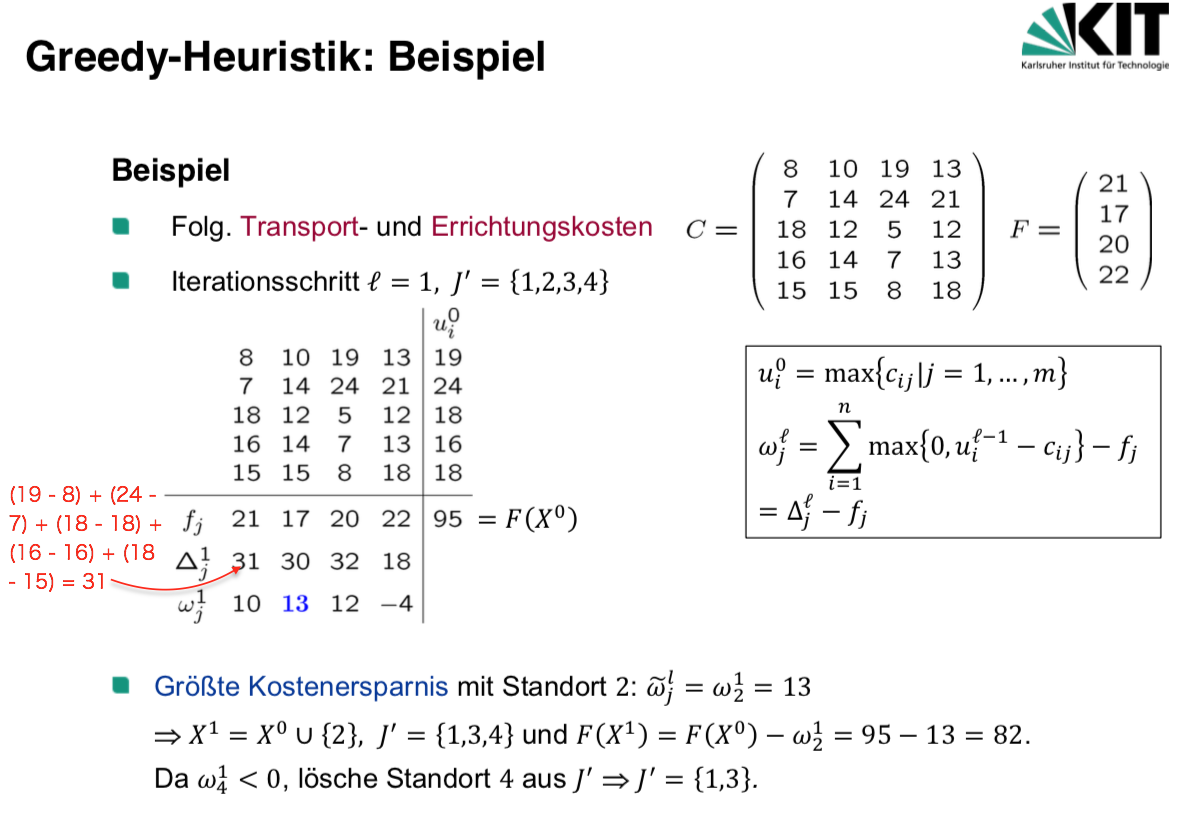
\includegraphics[width=0.95\textwidth]{Images/Greedy_Heuristik_Bsp(1).png}
          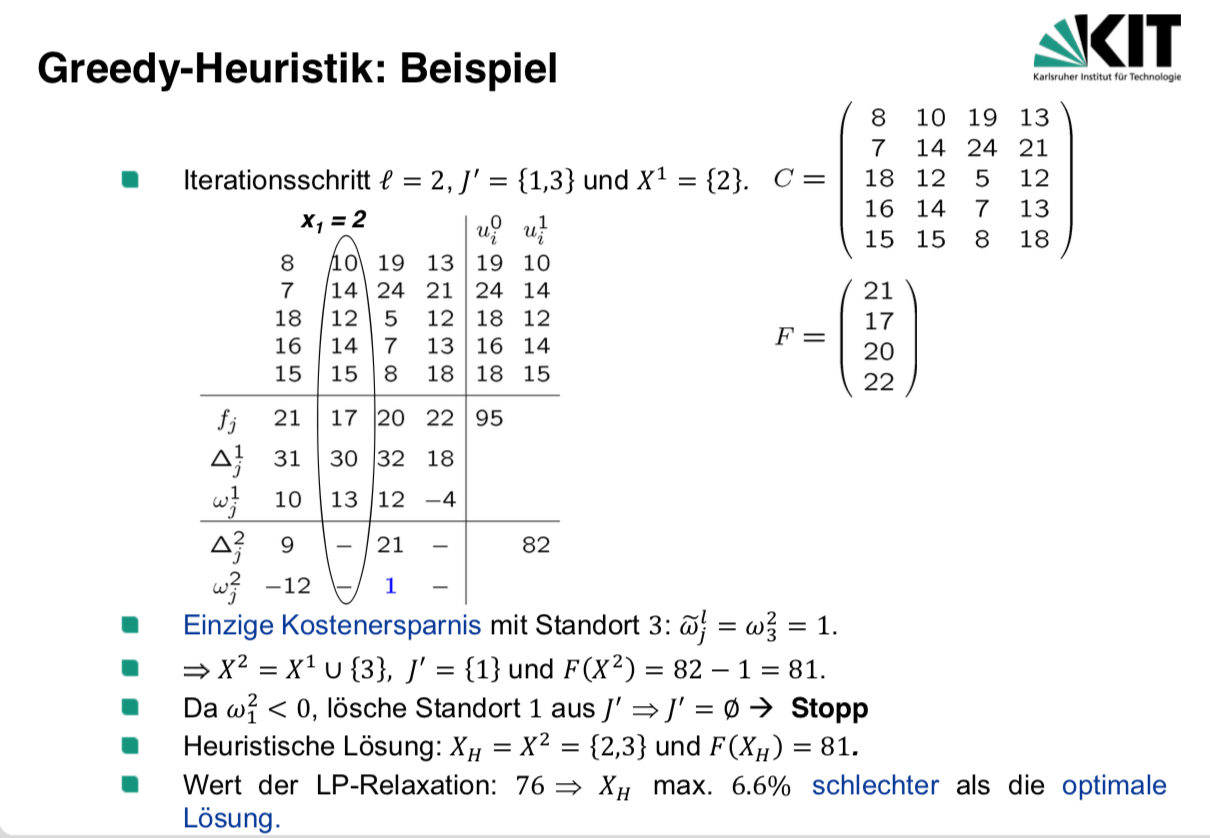
\includegraphics[width=0.95\textwidth]{Images/Greedy_Heuristik_Bsp(2).png}
          \caption{Greedy Heuristik Bsp}
          \label{fig:Greedy_Heuristik_Bsp}
        \end{figure}

        \begin{exmp}
          \color{blue}{Aufgabe 14}
        \end{exmp}

      \subsubsection{Interchange-Heuristik}

    % subsection heuristiken (end)

    \subsection{Das DUALOC-Verfahren} % (fold)
    \label{sub:das_dualoc_verfahren}

      \begin{figure}[H]
        \centering
        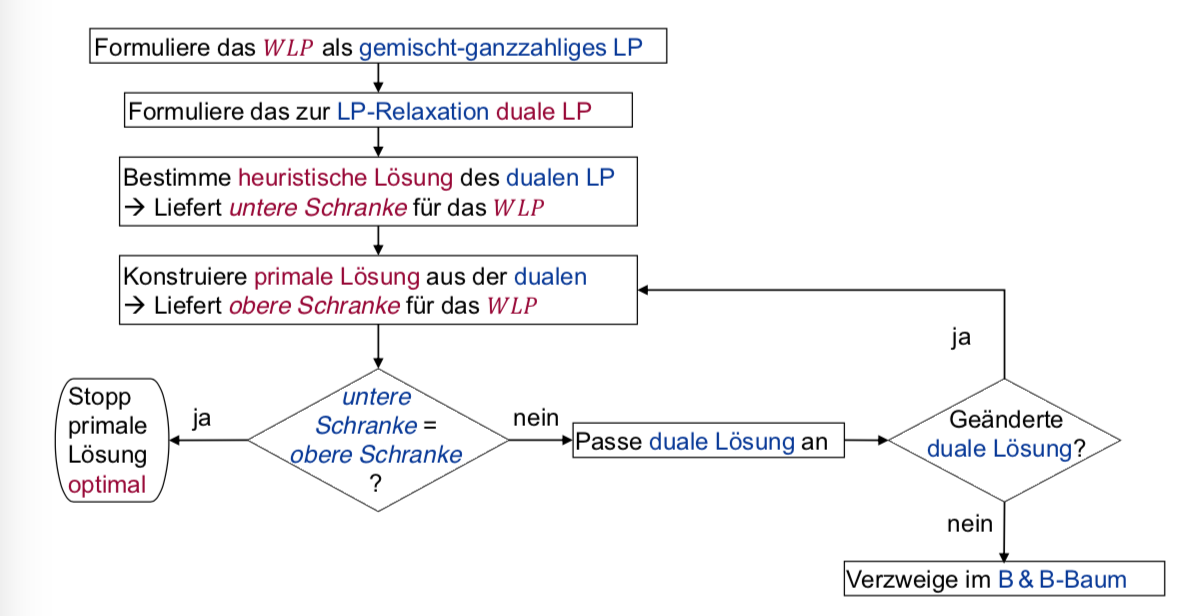
\includegraphics[width=0.95\textwidth]{Images/DUALOC_Verfahren.png}
        \caption{DUALOC-Verfahren}
        \label{fig:DUALOC_Verfahren}
      \end{figure}

      \begin{exmp}
          \color{blue}{Aufgabe 15, 16}
        \end{exmp}

      \par \textbf{1. WLP als gemischt-ganzzahliges lineares Programm}

      \begin{equation}
        \begin{aligned}
          & \underset{}{\text{min}}
          && \sum_{i=1}^{n}\sum_{j=1}^{m}c_{ij}x_{ij} + \sum_{j=1}^{m}f_jy_{j}\\
          % & & e - (s + re) \\
          & \text{u.d.N}
          & & \sum_{j=1}^{m}x_{ij}=1, \forall i \\
          & & & x_{ij} \leq y_j, \forall i, \forall j \\ 
          & & & x_{ij} \geq 0, y_j \in \{0,1\}, \forall i, \forall j \\
        \end{aligned}
      \end{equation}

      \par \textbf{LP-Relaxation (LP)} des gemischt-ganzzahligen linearen Programms für das WLP

      \begin{equation}
        \begin{aligned}
          & \underset{}{\text{min}}
          && \sum_{i=1}^{n}\sum_{j=1}^{m}c_{ij}x_{ij} + \sum_{j=1}^{m}f_ky_{j}\\
          % & & e - (s + re) \\
          & \text{u.d.N}
          & & \sum_{j=1}^{m}x_{ij}=1, \forall i \\
          & & & x_{ij} \leq y_j, \forall i, \forall j \\ 
          & & & x_{ij} \geq 0, y_j \geq 0, \forall i, \forall j \\
        \end{aligned}
      \end{equation}

      \par \textbf{2. duale lineare Programm (DP)} ) mit den Dual-Variablen $v_i$ und $w_{ij}$ 

      \begin{equation}
        \begin{aligned}
          & D(v, w) = \text{max}
          && \sum_{i=1}^{n}v_i\\
          % & & e - (s + re) \\
          & \text{u.d.N}
          & & \sum_{i=1}^{n}w_{ij} \leq f_j, \forall j \\
          & & & v_i - w_{ij} \leq c_{ij}, \forall i, \forall j \\
          & & & v_i \lessgtr 0, \forall i\\
          & & & w_{ij} \geq 0, \forall i, \forall j
        \end{aligned}
      \end{equation}

      \par \textbf{Reduziertes duales LP (RDP)}

      \begin{equation}
        \begin{aligned}
          & D(v, w) = \text{max}
          && \sum_{i=1}^{n}v_i\\
          % & & e - (s + re) \\
          & \text{u.d.N}
          & & \sum_{i=1}^{n}max\{0, v_i- c_{ij}\} \leq f_j, \forall j \\
          % & & & v_i - w_{ij} \leq c_{ij}, \forall i, \forall j \\
          & & & v_i \lessgtr 0, y_j \geq 0, \forall i
          % & & & w_{ij} \geq 0, \forall i, \forall j
        \end{aligned}
      \end{equation}

      \par 3. Löse das (RDP) mit dem \textbf{Dual Ascent-Verfahren} und erhalte eine heuristische Lösung von (DP). $\rightarrow$ liefert die untere Schranke für das (WLP).

      \subsection{Dual Ascent-Verfahren} % (fold)
      \label{sub:dual_ascent_verfahren}

        \par \textbf{Idee/Vorgehensweise}
        \par Erhöhe, ausgehend von einer Startlösung $v$, reihum jedes $v_i$ solange um einen kleinen Wert, bis keines mehr erhöht werden kann.

        \par Definiere:
        \begin{itemize}
          \item $J_i := \{j \in J | v_i \geq c_{ij}\}$
          \item $s_j := f_j - \sum_{i = 1}^{n}max\{0, v_i - c_{ij}\}, \forall j in J$
          \item $k(i) := min\{k|c_i^k \geq v_i\}$
        \end{itemize}

        \begin{algorithm}[H]
          \begin{algorithmic}[1]
            \caption{Dual Ascent-Verfahren}
            \State Init:
            \State Sortiere die Kostenelement $c_{ij}$ jedes Kunden $i \in I$ nach monoton zunehmenden Werten und bezeichne sie mit $c_i^k$: $c_i^1 \leq c_i^2 \leq \dots \leq c_i^m \leq c_i^{m+1}:= \infty$
            \State $I':= I, v_i := c_i^1$ für $\forall i \in I$
            \State Berechne $J_i := \{j \in J | v_i \geq c_{ij}\}, \forall i \in I$ und  $s_j := f_j - \sum_{i = 1}^{n}max\{0, v_i - c_{ij}\}, \forall j \in J$
            \State Bestimme $k(i) := min\{k|c_i^k \geq v_i\}, \forall i \in I$
            \If{($v_i = c_i^{k(i)}$)} 
              \State $k(i) := k(i) + 1$
            \EndIf
            \While{($I' \neq \varnothing$)}
              \State Für $\forall i \in I'$: Bestimme $\vartriangle_i := min\{s_j|j \in J_i\}$
              \If{($\vartriangle_i = 0$)}
                \State $I':=I' \setminus \{i\}$
                \State Wähle das nächste $i \in I'$
              \Else
                \State Setze $\vartriangle = min\{\vartriangle_i, c_i^{k(i)} - v_i\}$
                \If{($\vartriangle = \vartriangle_i$)}
                  \State $I' := I' \setminus \{i\}$
                \Else 
                  \State $k(i) := k(i) + 1$
                \EndIf
                \State Setze $v_i := v_i + \vartriangle$ 
                \State Für $\forall j \in J_i$, setze $s_j := s_j - \vartriangle$
                \State Aktualisiere $J_i$
              \EndIf
            \EndWhile
            \end{algorithmic}
          \textbf{Output:eine heuristische Lösung von (RDP) (Untere Schranke für das (WLP))} 
        \end{algorithm}

        \begin{exmp}
          
        \end{exmp}
      
        \begin{figure}[H]
          \centering
          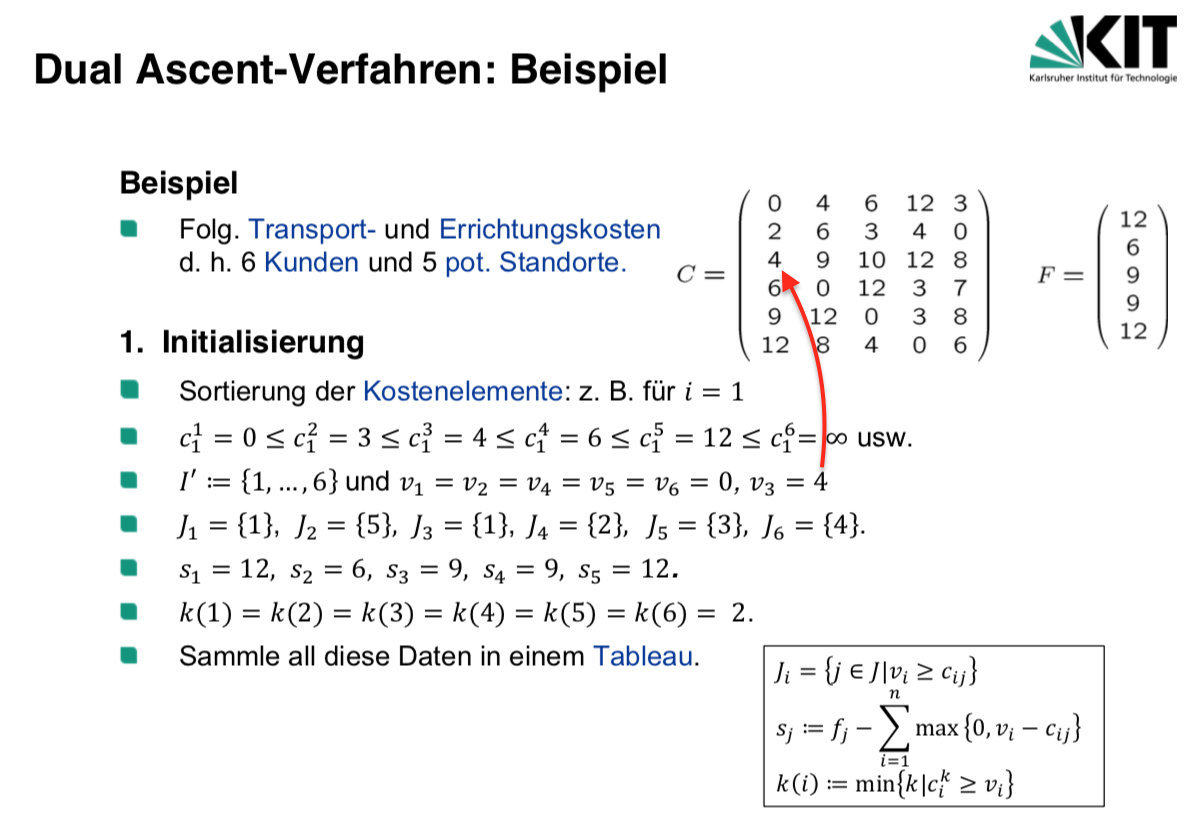
\includegraphics[width=0.95\textwidth]{Images/Dual_Ascent_Verfahrten_Bsp(1).png}
          \caption{Dual Ascent-Verfahren Bsp}
          \label{fig:dual_ascent_verfahren_bsp}
        \end{figure}

        \begin{figure}[H]
          \centering
          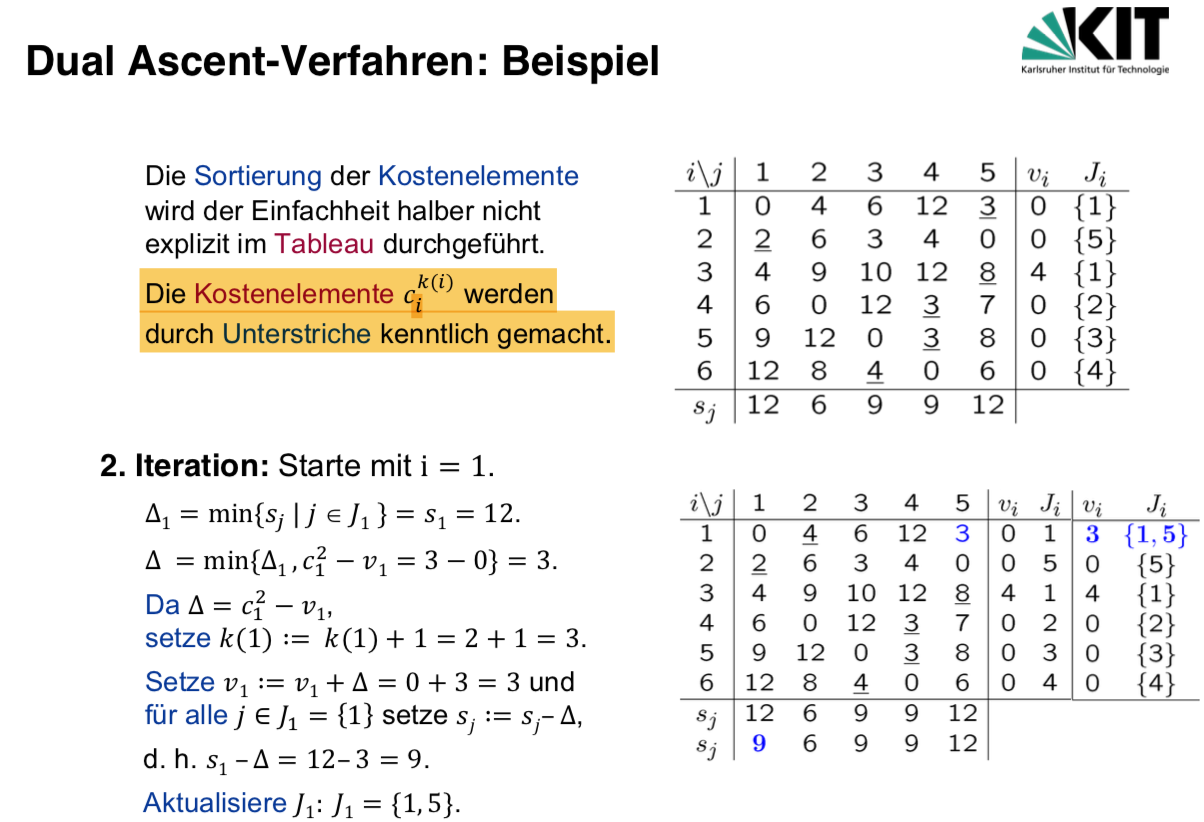
\includegraphics[width=0.95\textwidth]{Images/Dual_Ascent_Verfahrten_Bsp(2).png}
          \caption{Dual Ascent-Verfahren Bsp}
          \label{fig:dual_ascent_verfahren_bsp}
        \end{figure}

        \begin{figure}[H]
          \centering
          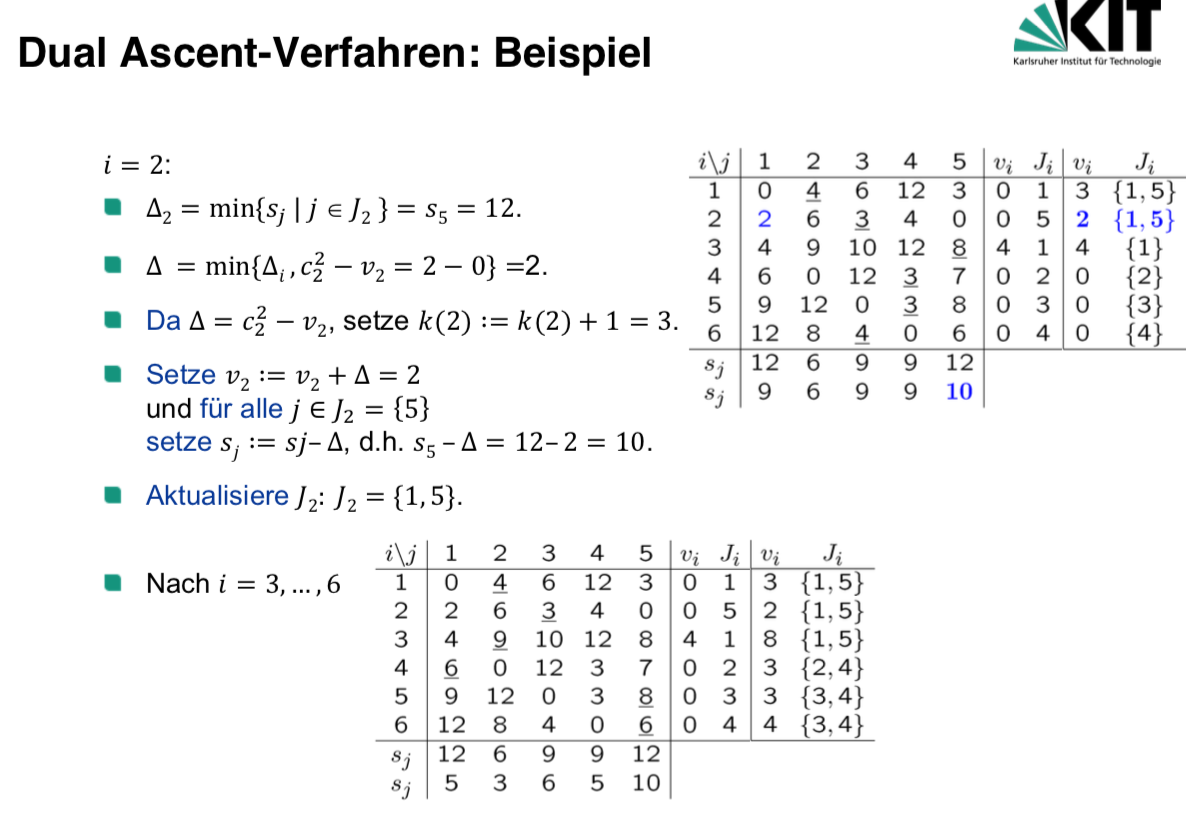
\includegraphics[width=0.95\textwidth]{Images/Dual_Ascent_Verfahrten_Bsp(3).png}
          \caption{Dual Ascent-Verfahren Bsp}
          \label{fig:dual_ascent_verfahren_bsp}
        \end{figure}

        \begin{figure}[H]
          \centering
          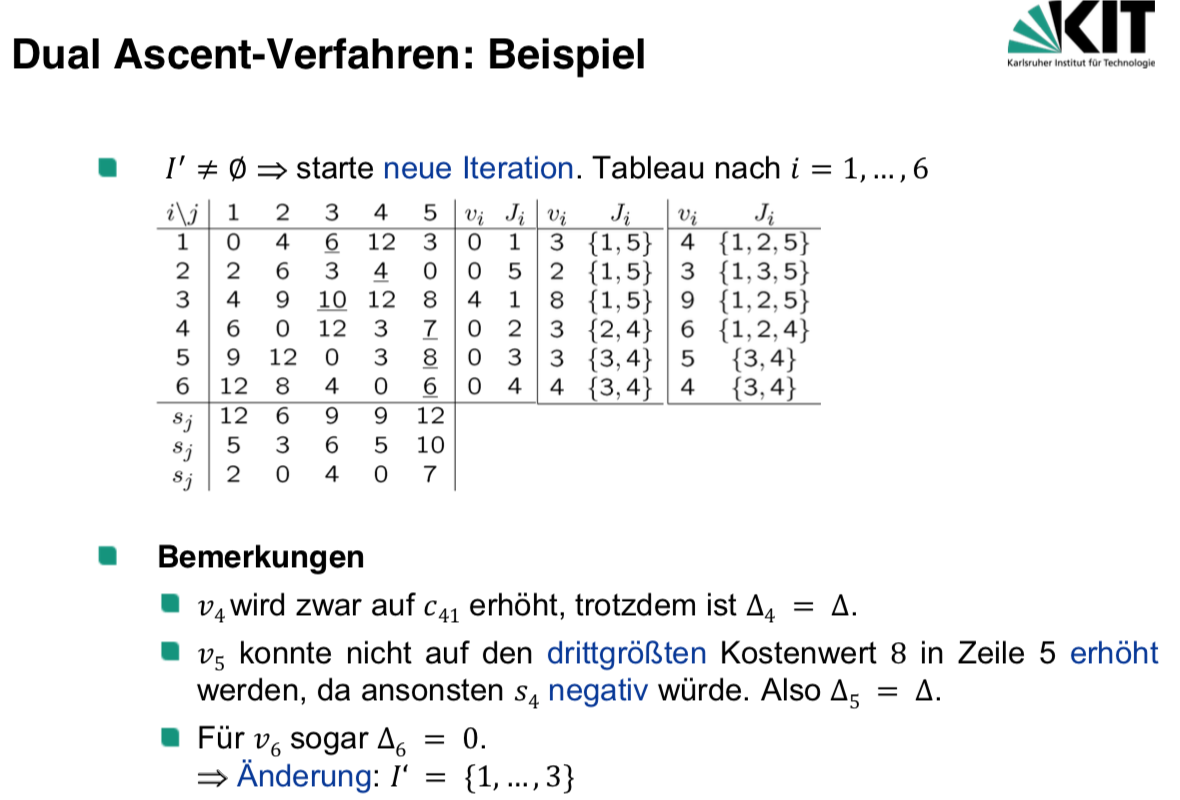
\includegraphics[width=0.95\textwidth]{Images/Dual_Ascent_Verfahrten_Bsp(4).png}
          \caption{Dual Ascent-Verfahren Bsp}
          \label{fig:dual_ascent_verfahren_bsp}
        \end{figure}

        \begin{figure}[H]
          \centering
          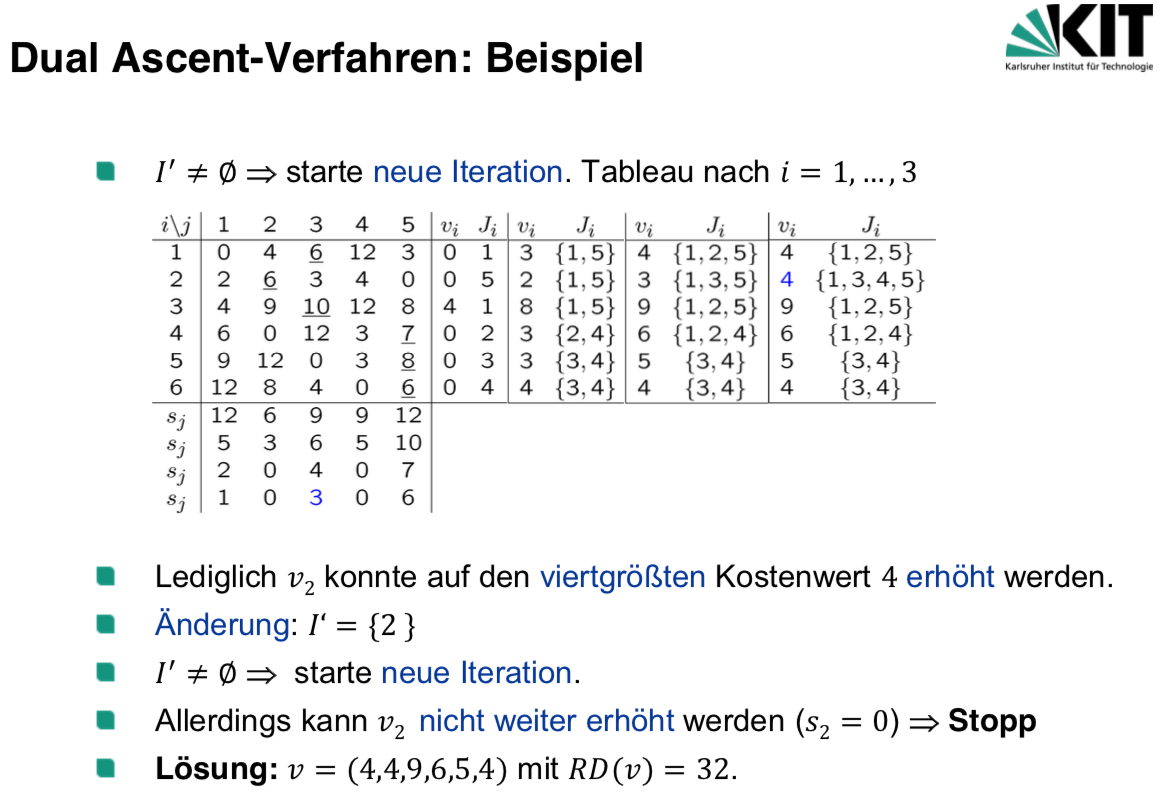
\includegraphics[width=0.95\textwidth]{Images/Dual_Ascent_Verfahrten_Bsp(5).png}
          \caption{Dual Ascent-Verfahren Bsp}
          \label{fig:dual_ascent_verfahren_bsp}
        \end{figure}
      % subsection dual_ascent_verfahren (end)


      \par 4. Konstruiere primär Lösung ausgehend von einer zulässinge Lösung $v$ von (RDP) mit \textbf{Konstruktionsheuristik} $\rightarrow$ liefert die obere Schranke für das (WLP)

      \subsection{Konstruktionsheuristik} % (fold)
      \label{sub:konstruktionsheuristik}

        \begin{algorithm}[H]
          \begin{algorithmic}[1]
            \caption{Konstruktionsheuristik}
            % \State \Comment{Init:}
            \State \textbf{Init}: setze $X = \varnothing$, berechne $J^+ = \{j \in J | s_j = 0\}$
            \State \textbf{Selektion von Standorten} 
            \State Für $\forall i \in I$: 
            \If{(Es gibt für Kunde $i$ genau einen Standort $j \in J^+$ mit $c_{ij} \leq v_i$ und $j \notin X$)}
              \State Setze $X = X \cup \{j\}, y_j = 1$
            \ElsIf{(Es gibt für Kunde $i$ mehrere Standorte $j \in J^+$ mit $c_{ij}, \leq v_i$ aber keines dieser $j \in X$)}
              \State setze $X = X \cup \{j^*\}, y_{j^*} = 1$ für das $j^*$ mit $c_{ij^*} = min\{c_{ij}|c_{ij} \leq v_i\}$
            \EndIf
            \State \textbf{Zuordnung}
            \State Ordne jeden Kunden $i$ dem kostengünstigsten Standort $j \in X$ zu:
            $x_{ij^*} = 1$ für das $j^*$ mit $c_{ij^*} = min\{c_{ij}|c_{ij} \leq v, j \in X\}$

            \end{algorithmic}
          \textbf{Output:primäre Lösung (obere Schranke für das (WLP))} 
        \end{algorithm}

        \begin{exmp}
          
        \end{exmp}

        \begin{figure}[H]
          \centering
          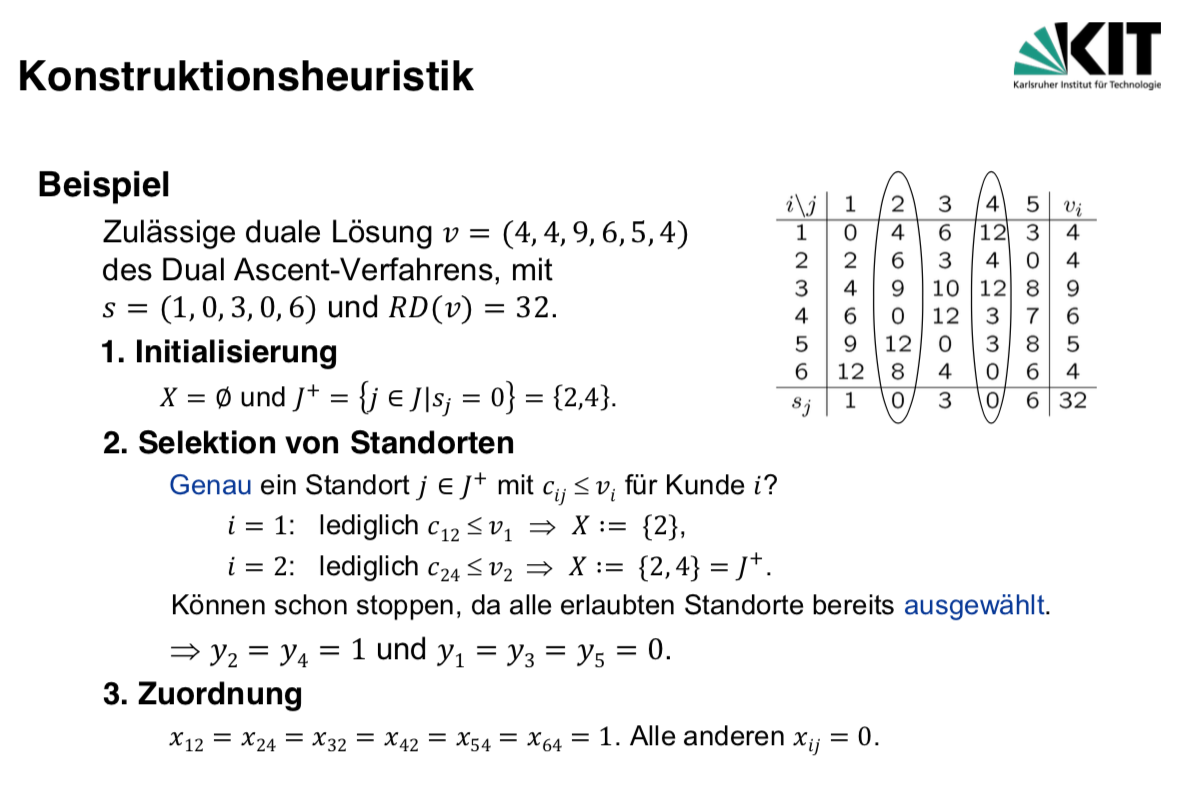
\includegraphics[width=0.95\textwidth]{Images/Konstruktionsheuristik_Bsp.png}
          \caption{Konstruktionsheuristik Bsp}
          \label{fig:Konstruktionsheuristik_Bsp}
        \end{figure}
      
      % subsection konstruktionsheuristik (end)

      \par 5. \textbf{Optimalitätsbedingungen} erfüllt?

      \begin{itemize}
        \item $s_j \geq 0 \Rightarrow y_j= 0; s_j=0 \Rightarrow y_j > 0$
        \item $v_i < c_{ij} \Rightarrow x_{ij} = 0; v_i \geq c_{ij} \Rightarrow x_{ij} \geq 0 $
        \item $v_i > c_{ij} \Rightarrow x_{ij} = y_j$
      \end{itemize}

      \par Falls die drei Bedingungen erfüllt sing $\rightarrow$ Die beide erhaltenen Lösung sind optimal
      \par Sonst $\rightarrow$ \textbf{Dual Adjustment Verfahren}, dann wieder Konstruktionsheuristik durchführen, bis die Optimalitätsbedingungen erfüllt werden. 
    

      \subsubsection{Dual Adjustment-Verfahren} % (fold)
      \label{ssub:dual_adjustment_verfahren}
      
        \par \textbf{Voraussetzung}
        \par zulässinge Lösungen $v$ von (RDP) und $(x, y)$ von (WLP).

        Definiere:
        \begin{itemize}
          \item $J_i^x := \{j \in X | v_i > c_{ij}\}$
          \item $c_{ij^*} = min\{c_{ij} | j \in J_i^x\}$
          \item $c_{ij^{**}} = min\{c_{ij} | j \in J_i^x, j \neq j^*\}$
          \item $I_J^x = \{i \in I | j \in X \text{ ist der einzige Standort mit } v_i \geq c_{ij}\}, j \in X$ 
        \end{itemize}
        
        

        \begin{algorithm}[H]
          \textbf{Input:} zulässinge Lösungen $v$ von (RDP) und $(x, y)$ von (WLP). (Nur für die Spalten mit $s_j = 0$ durchführen)
          \begin{algorithmic}[1]
            \caption{Dual Adjustment-Verfahren}
            \State \textbf{Iteration}
            \State Für $\forall i \in I$:
            \State Gilt $|J_i^x| \leq 1$ oder $I_{j^*}^x \cup I_{j**}^x = \varnothing$, so fahre mit dem nächsten $i$ fort.
            \State Bestimme das nächstkleinere $c_{ij}: \vartriangle := max\{c_{ij}|c_{ij} < v_i, j \in J\}$
            \State Setze $s_j := s_j + (v_i - \vartriangle)$ für $\forall j \in J_i^x$
            \State Setze $v_i:= \vartriangle$
            \State Führe das Dual Ascent-Verfahren nacheinander aus mit
            \begin{itemize}
              \item $I':=I_{j^*}^x \cup I_{j^{**}}^x$
              \item $I':= I' \cup \{i\}$
              \item $I':= I$
            \end{itemize}

            \end{algorithmic}
          % \textbf{Output:eine heuristische Lösung von (RDP)} 
        \end{algorithm}
      % subsubsection dual_adjustment_verfahren (end)

      \begin{exmp}
        
      \end{exmp}

      \begin{figure}[H]
        \centering
        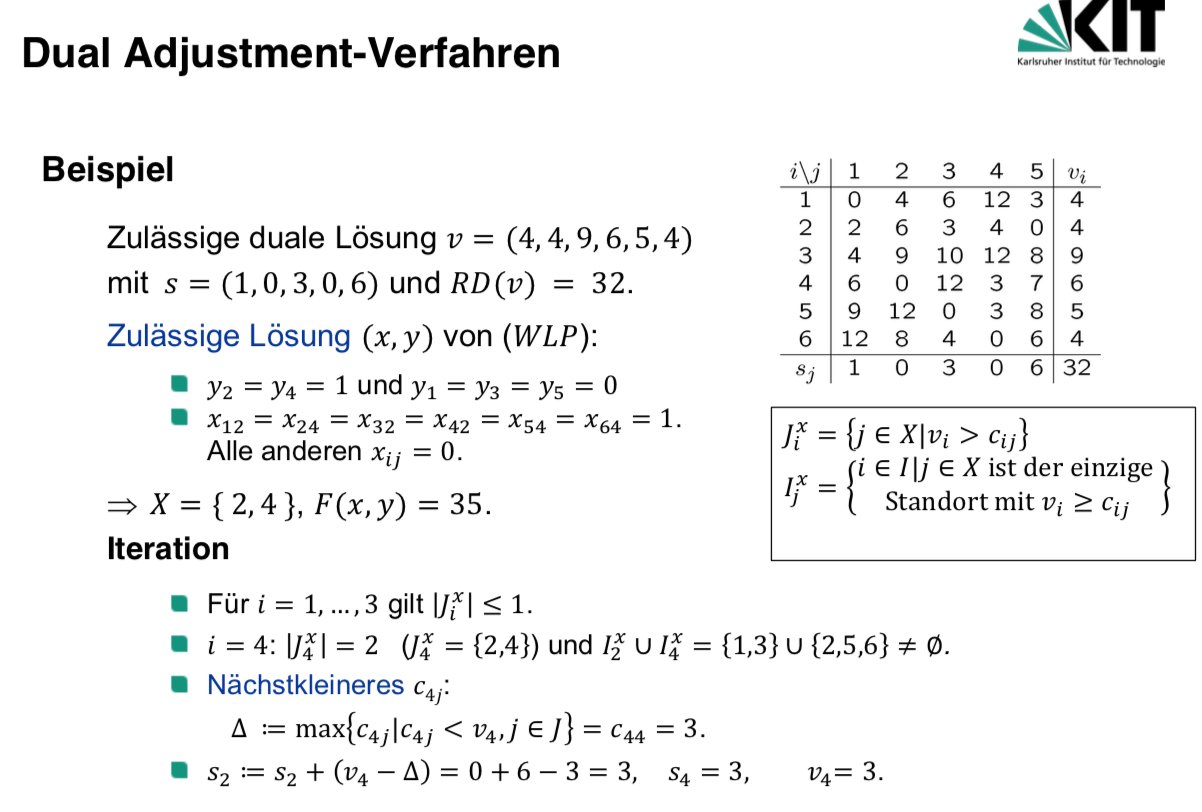
\includegraphics[width=0.95\textwidth]{Images/Dual_Adjustment_Verfahren_Bsp(1).png}
        \caption{Dual Adjustment-Verfahren Bsp}
        \label{fig:Dual_Adjustment_Verfahren}
      \end{figure}

      \begin{figure}[H]
        \centering
        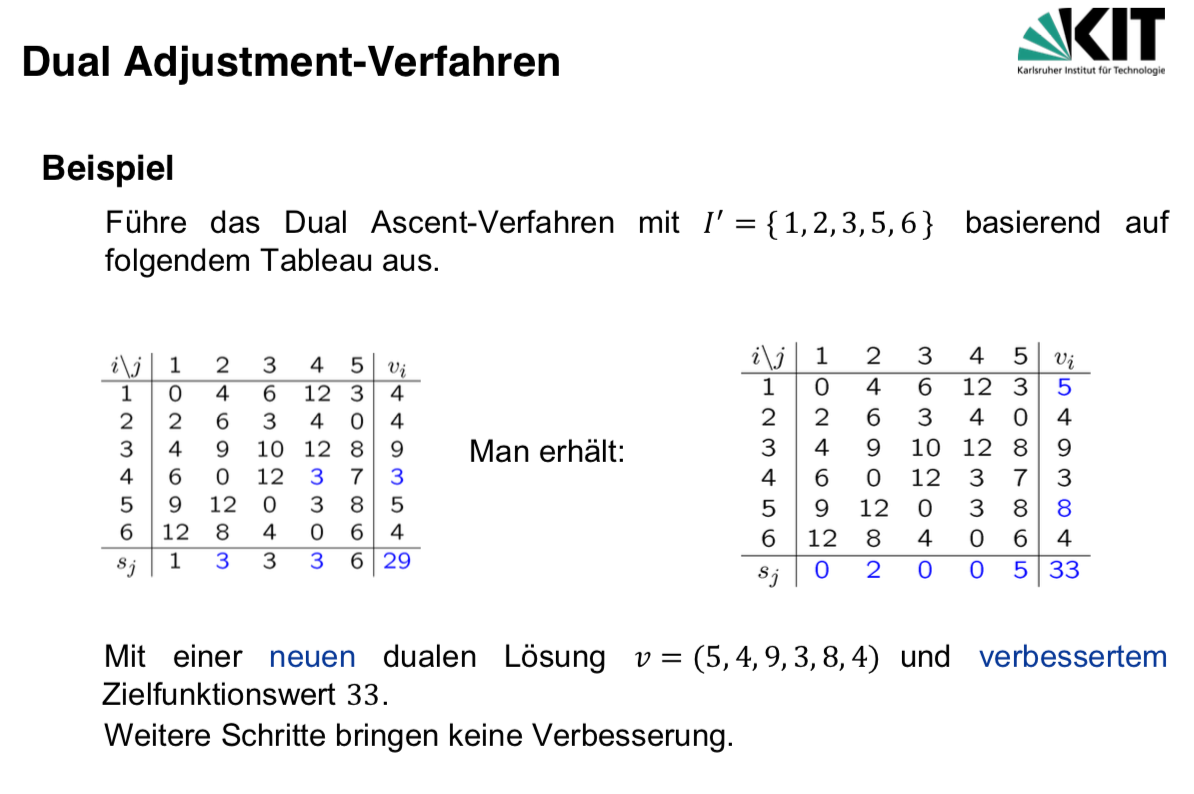
\includegraphics[width=0.95\textwidth]{Images/Dual_Adjustment_Verfahren_Bsp(2).png}
        \caption{Dual Adjustment-Verfahren Bsp}
        \label{fig:Dual_Adjustment_Verfahren}
      \end{figure}
    % subsection das_dualoc_verfahren (end)

    \begin{note}
      \begin{figure}[H]
        \centering
        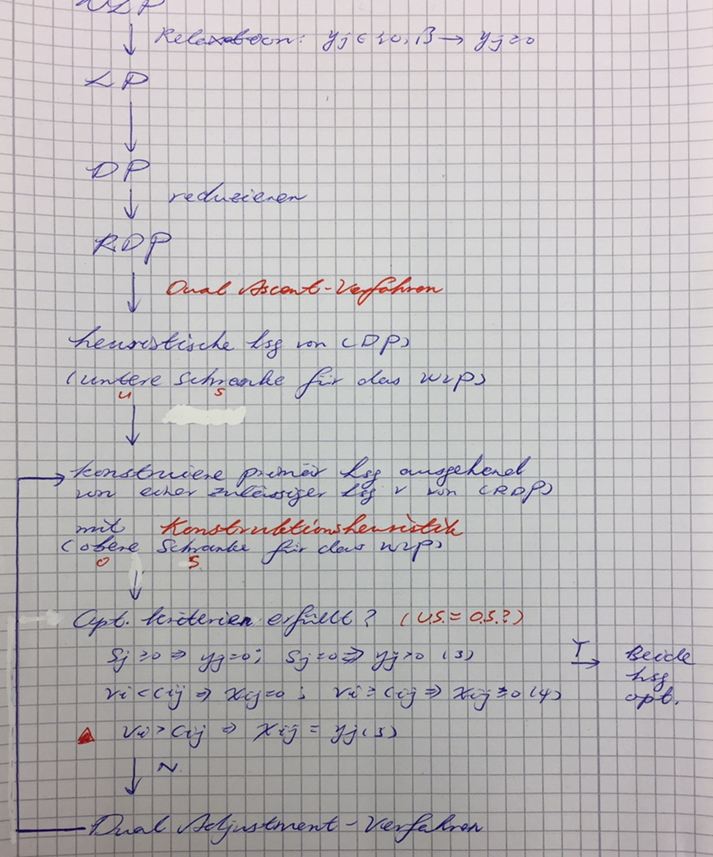
\includegraphics[width=0.95\textwidth]{Images/WLP_Zusammenfassung.JPG}
        \caption{WLP}
        \label{fig:WLP}
      \end{figure}
    \end{note}

  % section das_warehouse_location_problem_ (end)

  \section{Hub-Location-Probleme} % (fold)
  \label{sec:hub_location_probleme}
  
  % section hub_location_probleme (end)
% chapter diskrete_standortplanung (end)

    




  \chapter{Gebietsplanung} % (fold)
\label{cha:gebietsplanung}

  \par Ziel: kleine geographische Einheiten (sogenannte Basisgebiete) zu über- geordneten Gebieten (häufig als Bezirke, Cluster oder Territorien bezeichnet) unter der Berücksichtigung verschiedener relevanter Planungskriterien zusammenzufassen.

  \section{Basismodell} % (fold)
  \label{sec:basismodell}

    \subsection{Definitionen und Notationen} % (fold)
    \label{sub:definitionen_und_symbole}

      \par Ein Gebietsplanungsproblem umfasst eine Menge $V = \{1, \dots, M\}$ von Basisgebieten.

    \par Ein \textbf{Basisgebiet} $i \in V$ ist durch seinen Mittelpunkt $b_i = (x_i, y_i)$ bestimmt.

    \par Für jedes Basisgebiet $i \in V$ ist eine einzelne quantifizierbare Eigenschaft, das sogenannte \textbf{Aktivitätsmaß} $w_i$, gegeben. \\

    \par \textbf{Gebiet}:

    \begin{quote}
       \begin{itemize}
          \item Gebiete $D_1, \dots, D_p$ sind disjunkte Teilmengen der Basismenge, so dass jedes Basisgebiet in genau einem Gebiet enthalten ist:
            \begin{equation*}
              D_1 \cup \dots \cup D_p = V \quad \text{und} \quad D_i \cap D_j = \varnothing, i \neq j, b < p
            \end{equation*}
          
          \item Aktivitätsmaß oder die Größe eines Gebiets: die Summe der Aktivitätsmaße seiner Basisgebiete
            \begin{equation*}
              w(D_j) = \sum_{i \in D_j}w_i
            \end{equation*}

          \item \textbf{Zentrum} des Gebiets $j$: $c_j$ (Im Allgemeinen entspricht $c_j$ einem der Mittelpunkte der zum Gebiet $j$ gehörenden Basisgebiete.)
        \end{itemize}
    \end{quote}
     

    \par \textbf{\hl{Zusammenhang}}:

    Basisgebiet $b_i = (x_i, y_i) \in $ Menge der Basisgebiete $V \supseteq$ Gebiet $D_j$
    
    % subsection definitionen_und_symbole (end)

    \subsection{Modell-Kriterien} % (fold)
    \label{sub:modell_kriterien}
      
      \par \textbf{Balance}

      \par Alle Gebiete sollen balanciert sein, also möglichst gleich groß bzw. stark bezüglich der Aktivitätsmaße der Gebiete.

        \begin{quote}
          \begin{itemize}

            \item \textbf{perfekt balnciert} $\Leftrightarrow$ sein Aktivitätsmaß entspricht dem durchschnittlichen Aktivitätsmaß aller Gebiete $\mu$
            \begin{equation}
              \label{mu}
              w(D_j) = \mu = \frac{w(V)}{p}
            \end{equation}

            Auf Grund der diskreten Struktur des Problems können perfekt balancierte Vertriebsgebiete im Allgemeinen NICHT erzielt werden.

            \item \textbf{relative Abweichung} des Aktivitätsmaßes eines Gebiet
            \begin{equation*}
              bal(D_j) = \frac{|w(D_j) - \mu |}{\mu}
            \end{equation*}
          \end{itemize}
        \end{quote}
        

      \par \textbf{Kontiguität (Contiguity)}

      \par Zwei Basisgebiete werden als benachbart bezeichnet, wenn ihre geographischen Anordnungen nichtleere Schnittmengen besitzen.

      \par \textbf{Kompaktheit (Compactness)}

      \begin{quote}
        \begin{itemize}

          \item Reock-Test: Bilde das Verhältnis der Fläche des Gebiets zur Fläche des kleinsten, das Gebiet umschließenden Kreises.
          \begin{equation*}
            cp(D_j) = \frac{A_{A_j}}{A_{uk}} \leq 1
          \end{equation*}

          \item Schwartzberg-Test: Bilde das Verhältnis zwischen dem Umfang eines Kreises, der dadurch festgelegt ist, dass er den gleichen Flächeninhalt wie das Gebiet hat, und dem Umfangs des Gebiets.
          \begin{equation*}
            cp(D_j) = \frac{2 \cdot \sqrt{\pi \cdot A_{D_j}}}{U_{D_j}} \leq 1
          \end{equation*}

        \end{itemize}
      \end{quote}
        

        Je näher $cp(D_j)$ an 1, umso kompakter ist das Gebiet.

    % subsection modell_kriterien (end)

    \subsection{Ziel der Gebietsplanung} % (fold)
    \label{sub:ziel_der_gebietsplanung}

      \par Untergliedere alle Basisgebiete $V$ in $p$ Gebiete, welche die Planungskriterien der Balance, Kompaktheit, Kontiguität und Disjunktheit erfüllen.
    
    
    % subsection ziel_der_gebietsplanung (end)
    
  % section basismodell (end)

  \section{Vorgehensweisen zur Gebietsplanung} % (fold)
  \label{sec:vorgehensweisen_zur_gebietsplanung}

    \subsection{Notation} % (fold)
    \label{sub:notation}

      \begin{itemize}
        \item $V$: Menge der Basisgebiete
        \item $w_u$: Aktivitätsmaß des Basisgebiets $u$
        \item $p$: Anzahl der Gebiete
        \item $d_{uv}$: Distanzen
        \item $\mu$: Durchschnittsgröße bzgl. $w$ (\eqref{mu})
        \item $\tau$: Toleranz der Balance
        \item \begin{equation*}
                    x_{uv} = 
                    \begin{cases}
                      1 & \text{falls Basisgebiet } u \text{ einem Gebit mit dem Zentrum } v \text{ zugeordnet wird.} \\
                      0 & sonst
                    \end{cases}
                \label{trivial wage scheme}
            \end{equation*}
      \end{itemize}
    
    % subsection notation (end)

    \subsection{LP-Formulierung} % (fold)
    \label{sub:lp_formulierung}

      \begin{equation*}
        \begin{aligned}
          & \underset{u,v \in V}{\text{min}}
          & & d_{uv}^2w_{u}x_{uv}\\
          & \text{s.t.}
          & & \sum_{v \in V}x_{uv} = 1 & \quad (u \in V) \quad \text{(Vollst. Zuordnung)}\\ 
          & & & \mu(1 - \tau)x_{vv} \leq \sum_{u \in V}w_ux_{uv} \leq \mu(1 + \tau)x_{vv} &\quad  (v \in V)\quad \quad \text{(Balance)} \\
          & & &\sum_{v \in V}x_{vv} = p \qquad \qquad(p \text{ Gebiete})\\
          & & &x_{uv} \in \{0, 1\}  \qquad (u, v \in V)
        \end{aligned}
        \label{LEN principal problem}
      \end{equation*}
    
    % subsection lp_formulierung (end)
  
  % section vorgehensweisen_zur_gebietsplanung (end)

  \section{Recursive-Partitioning-Algorithmus} % (fold)
  \label{sec:recursive_partitioning_algorithmus}

    \par {\color{blue}{(Bsp: Aufgabe 19)}}

    \par \textbf{Grundidee}:
      \begin{itemize}
         \item Unterteile das Problem rekursiv auf geometrische Weise durch Linien in immer kleinere Teilprobleme.
         \item Wiederhole dies solange, bis eine elementare Größe erreicht ist, in welcher das Gebietsplanungsproblem in effizienter Zeit gelöst wird.
       \end{itemize} 

    \subsection{Definitionen} % (fold)
    \label{sub:definitionen}

      \par \textbf{Partionsproblem}

      \par $PP = (B, q)$ wird als Partitionsproblem bezeichnet, falls $B \subseteq V$ und $1 \leq q \leq p$ gilt.\\
    
      \par \textbf{Linienpartition}

      \par $LP = (B_l, B_r, q_l, q_r)$ wird als Linienpartition bezeichnet, falls:
        \begin{quote}
          \begin{enumerate}
            \item $B_l \cup b_r = B \text{und} B_l \cap B_r = \varnothing$
            \item $\exists \text{ Line } L: B_l = B \cap H^{\leq}(L) \text{ und } B_r = B \cap H^{>}(L)$
            \item $q \leq q_l, q_r \leq q \text{ und } q_l + q_r = q$
          \end{enumerate}
        \end{quote}
    % subsection definitionen (end)   

    \subsection{Recursive-Partitioning} % (fold)
    \label{sub:recursive_partitioning}

      \par \textbf{Gleichmäßige Aufteilung}:

        \begin{quote}
          \begin{itemize}
            \item $q_l = q_r = \frac{q}{2}$, falls $q$ gerade
            \item $q_l = \frac{q - 1}{2}, q_r = \frac{q + 1}{2}$ und $q_l = \frac{q + 1}{2}, q_r = \frac{q - 1}{2}$, falls $q$ ungerade
          \end{itemize}
        \end{quote}

      \par \textbf{Balance}:

      \begin{equation*}
        bal(LP) = \max \{ \frac{|\frac{w(B_L)}{q_l} - \mu|}{\mu}, \frac{|\frac{w(B_r)}{q_r} - \mu|}{\mu}\}
      \end{equation*}

      \par \textbf{Partionsposition}:

      \indent \par Bestimme $k'$, so dass $\frac{w(B_{l}^{k'})}{q_l} < \frac{w(B)}{q}$ und $\frac{w(B_{l}^{k' + 1})}{q_l} \geq \frac{w(B)}{q}$

      \begin{equation*}
        k^* = 
          \begin{cases}
            k' & \text{falls } \frac{w(B)}{q} - \frac{w(B_{l}^{k'})}{q_l} \leq \frac{w(B_{l}^{k' + 1})}{q_l} - \frac{w(B)}{q} \\
            k' + 1 &\text{sonst}
          \end{cases}
      \end{equation*}
    
      \par \textbf{Kompaktheit}:

      \begin{equation*}
        cp(LP) = d(c_1. c_2) = l_2(c_!, c_2)
      \end{equation*}

    % subsection recursive_partitioning (end)

    \subsection{Algorithmus} % (fold)
    \label{sub:algorithmus}

      \begin{algorithm}
        \caption{Recursive-Partitioning-Algorithmus}\label{Recursive-Partitioning-Algorithmus}
        \textbf{Input}: Anzahl Suchrichtungen $K, \beta, V, p$
        \begin{algorithmic}[1]
          % \Procedure{MyProcedure}{}
          \State Markiere Partitionsproblem $PP = (V, p)$ als ungelöst
          \While {es gibt ungelöste Probleme}:
            \State Wähle ein ungelöstes Problem $PP = (B, q)$
            
            \If {$q = 1$}
              \State füge $B$ der Lösungsmenge $DL$ hinzu und markiere $PP$ als gelöst
            \EndIf

            \If {$q > 1$}
              \State Bestimme für jede Suchrichtung die Linienpartition $LP(k^*)$ mit der besten Balance und füge sie einer Menge $FLP$ hinzu.
              \State Bewerte alle Linienpartitionen $LP$ der Menge $FLP$ durch:
              
                \begin{equation*}
                  rk(LP) = \beta\frac{bal(LP)}{bal^{max}} + (1 - \beta)\frac{cp(LP)}{cp^{max}}
                \end{equation*}

              \State Wähle $LP^{*} = (B_{l}^{*}, B_{r}^{*}, q_{l}^{*}, q_{r}^{*}) = \underset{LP \in FLP}{\text{min}}rk(FLP)$ 

              \State Erstelle Partitionsprobleme $PP_l = (B_{l}^{*}, q_{l}^{*})$ und $PP_r = (B_{r}^{*}, q_{r}^{*})$ und markiere sie als ungelöst, markiere $PP$ als gelöst.
            \EndIf
          \EndWhile
          % \EndProcedure
        \end{algorithmic}
        \textbf{Output:} Gebietslayout DL
      \end{algorithm}


    
    % subsection algorithmus (end)
        
       
  % section recursive_partitioning_algorithmus (end)


% chapter gebietsplanung (end)




    




  
      
 
\end{document}
